\subsection{凸函数的连续性与可导性}

命题 5. 为使实值有限函数 f 在区间 I 上是凸的（相应地，严格凸的），必须且只需：对一切 \(a \in I\)，梯度

\[
p (\mathbf {M} _ {a} \mathbf {M} _ {x}) = \frac {f (x) - f (a)}{x - a}
\]

在 I ∩ ∁\{a\} 上是 x 的递增（相应地，严格递增）函数。

本命题是定义 1 和定义 2 以及 I, p.~23 中的引理的直接推论。

命题 6. 设 \(f\) 是区间 \(\mathbf{I} \subset \mathbf{R}\) 上的实值有限凸函数。那么，在每个内点 \(a\)（属于 \(\mathbf{I}\)）处，函数 \(f\) 连续，具有有限的右导数与左导数，并且 \(f_g'(a) \leqslant f_d'(a)\)。

事实上，对 \(x \in I\) 与 \(x > a\)，函数 \(x \mapsto \frac{f(x) - f(a)}{x - a}\) 递增（命题 5）且有下界，因为若 \(y < a\) 与 \(y \in I\)，就有

\[
\frac {f (y) - f (a)}{y - a} \leqslant \frac {f (x) - f (a)}{x - a}\tag{5}
\]

（依命题 5）；因此这个函数在点 \(a\) 处有有限的右极限；换言之，\(f_d'(a)\) 存在且有限；再者，在 (5) 中令 \(x\) 趋于 \(a\)（\(x > a\)），便得到

\[
\frac {f (y) - f (a)}{y - a} \leqslant f _ {d} ^ {\prime} (a)\tag{6}
\]

对一切属于 I 的 \(y < a\) 成立。同理可证 \(f_{g}^{\prime}(a)\) 存在，且

\[
f _ {d} ^ {\prime} (a) \leqslant \frac {f (x) - f (a)}{x - a}\tag{7}
\]

对 \(x \in I\) 以及 x \textgreater{} a 成立。在这最后一个不等式中令 x 趋于 \(a (x > a)\)，就得到 \(f_{g}^{\prime}(a) \leqslant f_{d}^{\prime}(a)\)。点 a 处左导数与右导数的存在性显然保证 f 在该点连续。

推论 1. 设 \(f\) 是 I 上的凸（相应地，严格凸）函数；若 \(a\) 与 \(b\) 是 I 的两个内点且 \(a < b\)，则有（图~3）

\pandocbounded{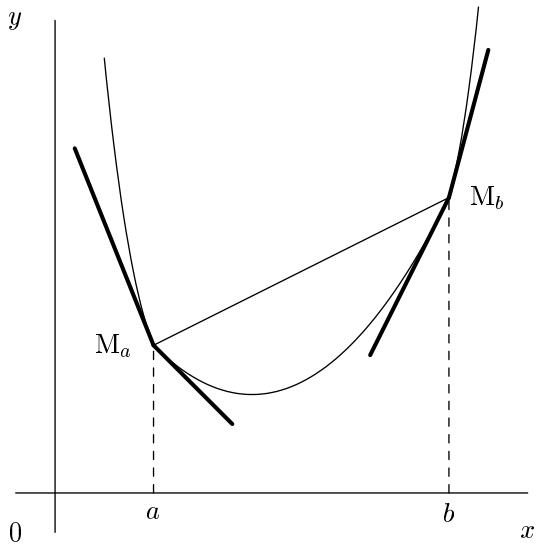
\includegraphics[keepaspectratio]{images/part001_a227d9e4.jpg}}\\
图 3

\[
f _ {d} ^ {\prime} (a) \leqslant \frac {f (b) - f (a)}{b - a} \leqslant f _ {g} ^ {\prime} (b)\tag{8}
\]

（相应地，

\[
f _ {d} ^ {\prime} (a) <   \frac {f (b) - f (a)}{b - a} <   f _ {g} ^ {\prime} (b)).\tag{9}
\]

二重不等式 (8) 由 (6) 与 (7) 经简单的记号改动而得。另一方面，若 \(f\) 严格凸，且 \(c\) 使得 \(a < c < b\)，则由 (8) 与命题 5 得

\[
f _ {d} ^ {\prime} (a) \leqslant \frac {f (c) - f (a)}{c - a} <   \frac {f (b) - f (a)}{b - a} <   \frac {f (b) - f (c)}{b - c} \leqslant f _ {g} ^ {\prime} (b)
\]

由此得 (9)。

推论 2. 若 f 在 I 上是凸的（相应地，严格凸的），则 \(f_{d}^{\prime}\) 与 \(f_{g}^{\prime}\) 在 I 的内部递增（相应地，严格递增）；I 中使 f 不可导的点所成的集是可数的，并且 \(f_{d}^{\prime}\) 与 \(f_{g}^{\prime}\) 在 f 可导的每一点处连续。

第一部分立即由 (8)（相应地，(9)）以及不等式

\[
f _ {g} ^ {\prime} (a) \leqslant f _ {d} ^ {\prime} (a).
\]

得出。另一方面，设 E 为 I 中使 f 不可导的内点 x 所成的集（即 \(f_{g}^{\prime}(x) < f_{d}^{\prime}(x)\)）。对每个 \(x \in E\)，设 \(J_{x}\) 为开区间 \(]f_{g}^{\prime}(x), f_{d}^{\prime}(x)[;\)；由 (8) 可知，若 x 与 y 是 E 中满足 x \textless{} y 的两点，则 u \textless{} v 对一切 \(u \in J_{x}\) 与一切 \(v \in J_{y}\) 成立；换言之，当 x 跑遍 E 时，非空开区间 \(J_{x}\) 两两不相交；这样的区间所成的集因此是可数的，从而 E 也是可数的。最后，\(f_{d}^{\prime}\)（相应地，\(f_{g}^{\prime}\)）递增，故它在 I 的每个内点 x 处都有右极限与左极限；于是 I, p.~18 的命题 6 表明，\(f_{d}^{\prime}\)（相应地，\(f_{g}^{\prime}\)）在点 x 处的右极限等于 \(f_{d}^{\prime}(x)\)，而其左极限等于 \(f_{g}^{\prime}(x)\)；由此即得推论的最后一部分。

设 \(f\) 是 \(I, a\) 上的凸函数，\(I\) 为其一个内点，\(D\) 为过点 \(M_a\) 的一条直线，其方程为 \(y - f(a) = \alpha(x - a)\)。由不等式 (8) 可知，若 \(f_g'(a) \leqslant \alpha \leqslant f_d'(a)\)，则图像 \(G\) 的每一点都位于 \(D\) 之上；并且若 \(f\) 严格凸，则 \(M_a\) 是 \(D\) 与 \(G\) 公有的唯一点；我们称 \(D\) 是 \(G\) 在点 \(M_a\) 处的一条支撑直线。反之，若 \(G\) 位于 \(D\) 之上，则 \(f(x) - f(a) \geqslant \alpha(x - a)\) 对每个 \(x \in I\) 成立，由此 \(\frac{f(x) - f(a)}{x - a} \geqslant \alpha\) 对 \(x > a\) 成立，\(\frac{f(x) - f(a)}{x - a} \leqslant \alpha\) 对 \(x < a\) 成立；在这些不等式中令 \(x\) 趋于 \(a\)，便得 \(f_g'(a) \leqslant \alpha \leqslant f_d'(a)\)。

特别地，若 \(f\) 在点 \(a\) 处可导，则 \(G\) 在点 \(M_a\) 处只有唯一一条支撑直线，即 \(G\) 在 \(M_a\) 处的切线。

注记。若 \(f\) 是开区间 \(I\) 上的严格凸函数，则 \(f_d'\) 在 \(I\) 上严格递增，于是根据 \(I\), p.~13 的命题 2，有三种可能的情形：

\(1^{\circ} f\) 在 I 上严格递减；

\(2^{\circ}\) f 在 I 上严格递增；

\(3^{\circ}\) 存在 \(a \in \mathrm{I}\)，使 \(f\) 对 \(x \leqslant a\) 严格递减，而对 \(x \geqslant a\) 严格递增。

当 \(f\) 在 \(I\) 上是凸的但非严格凸时，\(f\) 可以在含于 \(I\) 的某个区间上取常值；设 \(J = ]a, b[\) 为使 \(f\) 取常值的最大开区间（换言之，使 \(f_{d}^{\prime}(x)=0\) 的区间的内部）；那么 f 在由点 \(x\in I\)（满足 \(x\leqslant a\)）所成的区间上（若它存在）严格递减，在由点 \(x\in I\)（满足 \(x\geqslant b\)）所成的区间上（若它存在）严格递增。

在所有情形中都可以看出，\(f\) 在 I 的左端点处（在 \(\overline{\mathbf{R}}\) 中）具有右极限，在右端点处具有左极限；这些极限可以是有限的或无限的（参见~I, p.~46, 习题 5, 6 与 7）。在用语从宽的意义下，人们有时把取值于 \(\overline{\mathbf{R}}\)、在 I 的内部等于 \(f\) 且由连续性延拓到 I 的端点的连续函数说成是在 \(\overline{\mathbf{I}}\) 上凸的。

\subsection{凸性判别法}

命题 7. 设 f 是定义在区间 \(I \subset R\) 上的实值有限函数。为使 f 在 I 上是凸的，必须且只需：对 I 中满足 a \textless{} b 的每一对数 a, b，以及对每个实数 \(\mu\)，函数 \(f(x) + \mu x\) 都在点 a, b 之一处取得它在 \([a, b]\) 上的上确界。

此条件是必要的；事实上，由于 \(\mu x\) 在 \(\mathbf{R}\) 上凸，函数 \(f(x) + \mu x\) 在 I 上凸；因此可以只限于 \(\mu = 0\) 的情形。此时，对

\[
x = \lambda a + (1 - \lambda) b \quad (0 \leqslant \lambda \leqslant 1),
\]

有

\[
f (x) \leqslant \lambda f (a) + (1 - \lambda) f (b) \leqslant \operatorname{Max} (f (a), f (b)).
\]

此条件是充分的。取 \(\mu = -\frac{f(b) - f(a)}{b - a}\) 并设 \(g(x) = f(x) + \mu x\)；有 \(g(a) = g(b)\)，因此 \(g(x) \leqslant g(a)\) 对一切 \(x \in [a, b]\) 成立，并且可以立即验证这个不等式等价于把 (1) 中的 \(z\) 换成 \(a\)、\(x'\) 换成 \(b\) 所得的不等式。

命题 8. 为使实值有限函数 f 在开区间 \(I \subset R\) 上是凸的（相应地，严格凸的），必须且只需：它在 I 上连续，在此区间的某个可数子集相对于 I 的余集 B 的每一点处有导数，并且该导数在 B 上递增（相应地，严格递增）。

由命题 6 及其推论 2（I, p.~27），此条件是必要的；我们来证明它是充分的。因此假设 \(f'\) 在 B 上递增，而 \(f\) 不是凸的；于是存在（I, p.~27, 命题 5）I 的三个点 \(a, b, c\)，使得 \(a < c < b\) 且 \(\frac{f(c) - f(a)}{c - a} > \frac{f(b) - f(c)}{b - c}\)；但由中值定理（I, p.~14, 定理 1）有

\[
\frac {f (c) - f (a)}{c - a} \leqslant \sup _ {x \in \mathrm{B}, a <   x <   c} f ^ {\prime} (x) \quad \text { and } \quad \frac {f (b) - f (c)}{b - c} \geqslant \inf _ {x \in \mathrm{B}, c <   x <   b} f ^ {\prime} (x).
\]

于是有 \(\sup_{x\in \mathbf{B},a < x < c}f'(x) > \inf_{x\in \mathbf{B},c < x < b}f'(x)\)，这与 \(f'\) 在 B 上递增的假设矛盾。

若现在假设 \(f'\) 在 B 上严格递增，则 \(f\) 是凸的，且不可能在含于 I 的任何开区间上等于一个仿射线性函数，因为否则 \(f'\) 将在该区间上取常值，与假设矛盾。

推论。设 \(f\) 是区间 \(\mathbf{I} \subset \mathbf{R}\) 上的实值有限函数，连续且两次可导；为使 \(f\) 在 \(\mathbf{I}\) 上凸，必须且只需 \(f''(x) \geqslant 0\) 对一切 \(x \in \mathbf{I}\) 成立；为使 \(f\) 在 \(\mathbf{I}\) 上严格凸，必须且只需前述条件成立，并且使点 \(x \in \mathbf{I}\)（在其处 \(f''(x) > 0\)）所成的集在 \(\mathbf{I}\) 中稠密。

这由前一命题以及 I, p.~14 的推论立得。

例。*在区间 {]}0, +∞{[} 上，函数 \(x^r\)（r 为任意实数）的二阶导数等于 \(r(r - 1)x^{r - 2}\)；因此当 \(r > 1\) 或 \(r < 0\) 时它严格凸，而当 \(0 < r < 1\) 时严格凹。*

为了能表述凸性的另一个判别法，我们作如下定义：给定定义在区间 \(I \subset R\) 上的实值有限函数的图像 G 以及 I 的一个内点 a，则称过 \(M_{a} = (a, f(a))\) 的直线 D 局部在 G 上方（相应地，局部在 G 下方），若存在 a 的邻域 \(V \subset I\)，使 D 的每个含于 \(V \times R\) 的点都在 G 之上（相应地，之下）；则称 D 在点 \(M_{a}\) 处局部位于 G 上，若存在 a 的邻域 \(V \subset I\)，使 D 与 \(V \times R\) 的交等同于 G 与 \(V \times R\) 的交（换言之，若 D 同时局部在 G 上方且局部在 G 下方）。

命题 9. 设 f 是开区间 \(I \subset R\) 上的上半连续的实值有限函数。为使 f 在 I 上凸，必须且只需：对 f 的图像 G 的每个点 \(M_{x}\)，在该点处局部在 G 上方的每条直线都局部位于 G 上（在点 \(M_{x}\) 处）。

此条件是必要的：事实上，若 \(f\) 在 \(I\) 上凸，则在点 \(\mathbf{M}_a\)（属于 \(G\)，即 \(f\) 的图像）处都存在一条直线 \(\Delta\)，它支撑 \(G\)；而 \(\Delta\) 位于 \(G\) 之下，故更加局部位于 \(G\) 之下（I, p.~29）；若一条直线 \(D\) 局部在 \(G\) 之上（在点 \(\mathbf{M}_a\) 处），它就局部在 \(\Delta\) 之上，从而必与 \(\Delta\) 重合，因而局部位于 \(G\) 上（在点 \(\mathbf{M}_a\) 处）。

此条件是充分的。事实上，设它成立，并设 \(f\) 在 I 上不凸；于是存在 I 的两个点 \(a, b\)（\(a < b\)），使得有 G 的点 \(\mathbf{M}_x\) 严格位于线段 \(\mathbf{M}_a\mathbf{M}_b\) 之上（图~4）。换言之，函数 \(g(x) = f(x) - f(a) - \frac{f(b) - f(a)}{b - a} (x - a)\) 取值 \(>0\) 于 {[}a, b{]} 上；由于 \(g\) 在这个紧区间上有限且上半连续，它的上确界 \(k\)（在 {[}a, b{]} 上）有限，并且 \(>0\)，而且

\pandocbounded{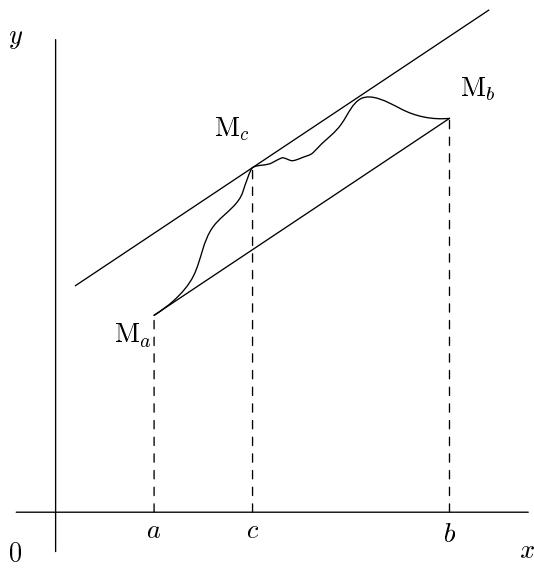
\includegraphics[keepaspectratio]{images/part001_3bcb0893.jpg}}\\
图 4

集 \(\overline{g}(k)\) 是闭的且非空（Gen.~Top., IV, p.~361, 定理 3 与命题 1）。设 c 是 \(\overline{g}(k)\) 的下确界；我们有 a \textless{} c \textless{} b，并且在点 \(M_{c}\) 处方程为 \(y = f(c) + \frac{f(b) - f(a)}{b - a}(x - c)\) 的直线 D 局部在 G 之上；但它在这一点不可能局部位于 G 上，因为对 a \textless{} x \textless{} c 有 \(g(x) < k\)，这表明 \(M_{x}\) 严格位于 D 之下。这就使我们得到矛盾，从而命题得证。

推论 1. 设 \(f\) 是定义在开区间 \(\mathbf{I} \subset \mathbf{R}\) 上且在 \(\mathbf{I}\) 上上半连续的实值有限函数；为使它在 \(\mathbf{I}\) 上凸，必须且只需：对一切 \(x \in \mathbf{I}\)，存在 \(\varepsilon > 0\)，使得关系 \(|h| \leqslant \varepsilon\) 蕴涵

\[
f (x) \leqslant \frac {1}{2} (f (x + h) + f (x - h)).
\]

我们只需证明此条件是充分的。事实上，若在 f 的图像 G 的某个点 \(M_{a}\) 处一条直线 D 局部在 G 之上，则它在该点处局部位于 G 上；因为若不然，例如，将有一个点 \(M_{a+h}\) 严格位于 D 之下，而一个点 \(M_{a-h}\) 位于 D 之下；于是线段 \(M_{a-h}M_{a+h}\) 的中点将严格位于 D 之上（图~5），而依假设，\(M_{a}\) 更加将严格位于 D 之下，这是荒谬的。

\pandocbounded{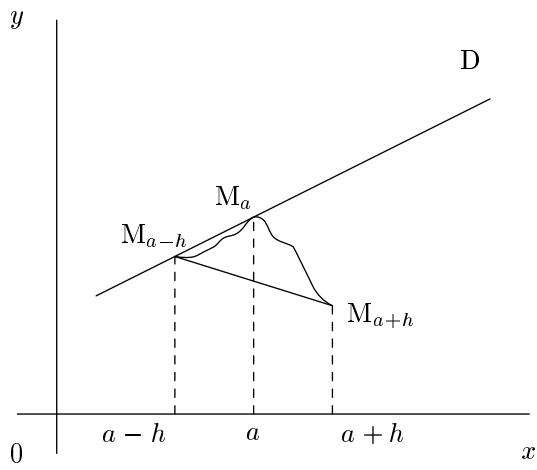
\includegraphics[keepaspectratio]{images/part001_b7dc5930.jpg}}\\
图 5

推论 2. 设 \(f\) 是定义在开区间 \(\mathrm{I} \subset \mathbf{R}\) 上的实值有限函数。若对每个点 \(x \in \mathrm{I}\) 都存在一个开区间 \(\mathrm{J}_x \subset \mathrm{I}\)，它包含 \(x\)，使 \(f\) 在 \(\mathrm{J}_x\) 上的限制在 \(\mathrm{J}_x\) 上凸，则 \(f\) 在 \(\mathrm{I}\) 上凸。

显然 \(f\) 满足命题 9 的判别法。

\setcounter{exercisegroup}{0}
\refstepcounter{exercisegroup}
\section*{第 \S\arabic{exercisegroup} 节习题}
\phantomsection
\addcontentsline{toc}{section}{第 \protect\S\arabic{exercisegroup} 节习题}

\begin{enumerate}
\def\labelenumi{\arabic{enumi})}
\tightlist
\item
  设 \(f\) 是定义在区间 \(I \subset \mathbf{R}\) 上的实变向量函数，在内点 \(x_0\)（\(I\) 的）处可导。证明商
\end{enumerate}

\[
\frac {f (x _ {0} + h) - f (x _ {0} - k)}{h + k}
\]

趋于 \(f'(x_0)\)（当 \(h\) 与 \(k\) 保持取值 \(> 0\) 而趋于 0 时）。逆命题。

*证明函数 \(f\)——等于 \(x^2 \sin 1/x\)（对 \(x \neq 0\)）且等于 0（对 \(x = 0\)）——处处可导，但 \((f(y) - f(z)) / (y - z)\) 并不趋于 \(f'(0)\)（当 \(y\) 与 \(z\) 在保持互异且 \(>0_*\) 的条件下趋于 0 时）。

\begin{enumerate}
\def\labelenumi{\arabic{enumi})}
\setcounter{enumi}{1}
\tightlist
\item
  在区间 I = {[}0, 1{]} 上，我们归纳地定义一个连续实函数序列 \((f_{n})\) 如下：取 \(f_{0}(x) = x\)；对每个整数 \(n \geqslant 1\)，函数 \(f_{n}\) 在 \(3^{n}\) 个区间 \(\left[\frac{k}{3^{n}}, \frac{k+1}{3^{n}}\right]\)（对于 \(0 \leqslant k \leqslant 3^{n}-1\)）的每一个上都是仿射线性的；此外，取
\end{enumerate}

\[
f _ {n + 1} \left(\frac {k}{3 ^ {n}}\right) = f _ {n} \left(\frac {k}{3 ^ {n}}\right)
\]

\[
f _ {n + 1} \left(\frac {k}{3 ^ {n}} + \frac {1}{3 ^ {n + 1}}\right) = f _ {n} \left(\frac {k}{3 ^ {n}} + \frac {2}{3 ^ {n + 1}}\right), f _ {n + 1} \left(\frac {k}{3 ^ {n}} + \frac {2}{3 ^ {n + 1}}\right) = f _ {n} \left(\frac {k}{3 ^ {n}} + \frac {1}{3 ^ {n + 1}}\right).
\]

证明序列 \((f_{n})\) 在 I 上一致收敛于一个连续函数，它在区间 {]}0, 1{[} 的任何点上都没有导数（有限的或无限的）（利用习题 1）。

\begin{enumerate}
\def\labelenumi{\arabic{enumi})}
\setcounter{enumi}{2}
\item
  设 \(\mathcal{C}(\mathrm{I})\) 是定义在紧区间 \(\mathrm{I} = [a,b]\)（含于 \(\mathbf{R}\)）上的连续实值有限函数所成的完备空间，并给 \(\mathcal{C}(\mathrm{I})\) 赋予一致收敛拓扑（Gen.~Top., X, p.~277）。设 A 是 \(\mathcal{C}(\mathrm{I})\) 中由满足如下条件的函数 \(x\) 组成的子集：至少存在一点 \(t\in [a,b[\)（依赖于函数 \(x\)），使函数 \(x\) 在该点有有限的右导数。证明 A 是 \(\mathcal{C}(\mathrm{I})\) 中的瘦集（Gen.~Top., IX, p.~192），因而其余集，即在 \([a,b[\) 的任何一点都没有有限右导数的连续函数所成之集，是 \(\mathcal{C}(\mathrm{I})\) 的一个贝尔子空间（Gen.~Top., IX, p.~192）。（设 \(\mathrm{A}_n\) 是由这样的函数 \(x\in \mathcal{C}(\mathrm{I})\) 组成的集：至少存在 \(t\) 的一个值，满足 \(a\leqslant t\leqslant b - 1 / n\)（且依赖于 \(x\)），使得 \(|x(t') - x(t)|\leqslant n|t' - t|\) 对 \(t'\) 的每个满足 \(t\leqslant t'\leqslant t + 1 / n\) 的值都成立。证明每个 \(\mathrm{A}_n\) 都是 \(\mathcal{C}(\mathrm{I})\) 中的闭的无处稠密集：注意在 \(\mathcal{C}(\mathrm{I})\) 中每个球都含有一个在 \([a,b[\) 上具有有界右导数的函数；另一方面，对每个 \(\varepsilon >0\) 和每个整数 \(m > 0\)，I 上存在一个连续函数，它在 \([a,b[\) 的每一点都有有限右导数，使得对一切 \(t\in [a,b[\) 有 \(|y(t)|\leqslant \varepsilon\) 与 \(|y_r'(t)|\geqslant m\)。）
\item
  设 E 是 R 上的拓扑向量空间，f 是定义在开区间 \(I \subset R\) 上的连续向量函数，并且在 I 的每一点都有右导数与左导数。
\end{enumerate}

\begin{enumerate}
\def\labelenumi{\alph{enumi})}
\item
  设 U 是 E 中的非空开集，A 是 I 中由满足 \(\mathbf{f}_{d}^{\prime}(x) \in \mathrm{U}\) 的点 x 组成的子集。给定数 \(\alpha > 0\)，设 B 是 I 中由这样的点 x 组成的子集：至少存在一个 \(y \in I\)，满足条件 \(x - \alpha \leqslant y < x\) 与 \((\mathbf{f}(x) - \mathbf{f}(y)) / (x - y) \in \mathrm{U}\)；证明集 B 是开集，并且 \(A \cap CB\) 是可数的（注意后一集由与 CB 邻接的区间的左端点组成）。由此推出，由点 \(x \in A\)（满足 \(\mathbf{f}_{g}^{\prime}(x) \notin \overline{\mathbf{U}}\)）所成的集是可数的。
\item
  假设 E 是赋范空间；这时像 \(\mathbf{f}(\mathrm{I})\) 是具有可数基的度量空间，对由 \(\mathbf{f}(\mathrm{I})\) 生成的 E 的闭向量子空间 F 亦然，该子空间包含 \(\mathbf{f}_{d}^{\prime}(\mathrm{I})\) 与 \(\mathbf{f}_{g}^{\prime}(\mathrm{I})\)。由 a) 推出，由点 \(x \in I\)（满足 \(\mathbf{f}_{d}^{\prime}(x) \neq \mathbf{f}_{g}^{\prime}(x)\)）所成的集是可数的。（若 \((\mathrm{U}_{m})\) 是 F 的拓扑的一个可数基，则注意对 F 的两个不同的点 a, b，存在两个不相交的集 \(U_{p}, U_{q}\)，使得 \(a \in U_{p}\) 与 \(b \in U_{q}\)。）
\item
  取 E 为乘积 \(R^{I}\)（即从 I 到 R 的映射所成的空间，赋予简单收敛拓扑），并对每个 \(x \in I\)，用 \(\mathbf{g}(x)\) 表示从 I 到 R 的映射 \(t \mapsto |x - t|\)。证明 g 连续，并且对每个 \(x \in I\) 有 \(\mathbf{g}_{r}'(x) \neq \mathbf{g}_{l}'(x)\)。
\end{enumerate}

\begin{enumerate}
\def\labelenumi{\arabic{enumi})}
\setcounter{enumi}{4}
\tightlist
\item
  设 \(\mathbf{f}\) 是定义在开区间 \(\mathrm{I} \subset \mathbf{R}\) 上、取值于一个赋范空间 \(\mathrm{E}\)（在 \(\mathbf{R}\) 上）中的连续向量函数，并且在 \(\mathrm{I}\) 的每一点处都有右导数。
\end{enumerate}

\begin{enumerate}
\def\labelenumi{\alph{enumi})}
\item
  证明满足如下条件的点 \(x \in \mathrm{I}\) 所成的集——\(\mathbf{f}_d'\) 在 \(x\) 的一个邻域上有界——是 \(\mathrm{I}\) 中的稠密开集（利用 Gen.~Top., IX, p.~194 的定理 2）。
\item
  证明 I 中使 \(\mathbf{f}_d^{\prime}\) 连续的点所成的集是 I 的一个瘦子集的余集（参见~Gen.~Top., IX, p.~255, 习题 21）。
\end{enumerate}

\begin{enumerate}
\def\labelenumi{\arabic{enumi})}
\setcounter{enumi}{5}
\tightlist
\item
  设 \((r_n)\) 是由 {[}0, 1{]} 中的有理数按某个次序排列而成的序列。证明函数 \(f(x) = \sum_{n=0}^{\infty} 2^{-n}(x - r_n)^{1/3}\) 连续且可导
\end{enumerate}

在 \(\mathbf{R}\) 的每个点处，并且在每个点 \(r_n\) 处有无穷导数。（为看出 \(f\) 在点 \(x\)（异于诸 \(r_n\)）处可导，分两种情形讨论，视通项为 \(2^{-n}(x - r_n)^{-2/3}\) 的级数的和是 \(+\infty\) 还是收敛而定；在第二种情形，注意对一切 \(x \neq 0\) 与一切 \(y \neq x\) 有

\[
0 \leqslant (y ^ {1 / 3} - x ^ {1 / 3}) / (y - x) \leqslant 4 / 3 x ^ {2 / 3}).
\]

\begin{enumerate}
\def\labelenumi{\arabic{enumi})}
\setcounter{enumi}{6}
\item
  设 \(f\) 是定义在区间 \(\mathrm{I} \subset \mathbf{R}\) 上的实函数，具有右导数 \(f_d'(x_0) = 0\)（在 \(\mathrm{I}\) 的一点处）；又设 \(\mathbf{g}\) 是定义在 \(y_0 = f(x_0)\) 的一个邻域上的向量函数，在该点处具有右导数与左导数（未必相等）。证明 \(\mathbf{g} \circ f\) 在点 \(x_0\) 处有等于 0 的右导数。
\item
  设 \(f\) 是从 \(\mathbf{R}\) 到其自身的映射，使得集 \(C\)（由 \(\mathbf{R}\) 中使 \(f\) 连续的点组成）在 \(\mathbf{R}\) 中稠密，并且 \(A\)（\(C\) 的余集）也稠密。证明集 \(D\)（由 \(C\) 中使 \(f\) 右可导的点组成）是瘦集。（对每个整数 \(n\)，设 \(E_n\) 是由这样的点 \(a \in \mathbf{R}\) 组成的集：存在两个点 \(x, y\)，使得 \(0 < x - a < 1/n\)、\(0 < y - a < 1/n\) 并且
\end{enumerate}

\[
\frac {f (x) - f (a)}{x - a} - \frac {f (y) - f (a)}{y - a} > 1.
\]

证明 \(E_{n}\) 的内部在 R 中稠密。为此，注意对 R 中每个非空开区间 I 都存在一点 \(b \in I \cap A\)；证明当 a \textless{} b 且 b - a 充分小时有 \(a \in E_{n}\)。

\begin{enumerate}
\def\labelenumi{\arabic{enumi})}
\setcounter{enumi}{8}
\tightlist
\item
  设 \(\mathcal{B}(\mathbf{N})\) 是实数的有界序列 \(\mathbf{x} = (x_n)_{n\in \mathbb{N}}\) 所成的空间，赋予范数 \(\| \mathbf{x}\| = \sup |x_n|\)；给出连续映射 \(t\mapsto \mathbf{f}(t) = (f_n(t))_{n\in \mathbb{N}}\)（从 \(\mathbf{R}\) 到 \(\mathcal{B}(\mathbf{N})\) 中）的一个例子，使得每个函数 \(f_{n}\) 在 \(t = 0\) 处可导，但 \(\mathbf{f}\) 在该点不可导。
\end{enumerate}

\setcounter{exercisegroup}{1}
\refstepcounter{exercisegroup}
\section*{第 \S\arabic{exercisegroup} 节习题}
\phantomsection
\addcontentsline{toc}{section}{第 \protect\S\arabic{exercisegroup} 节习题}

\begin{enumerate}
\def\labelenumi{\arabic{enumi})}
\item
  设 \(f\) 是定义在开区间 \(I = ]a, b[\)（含于 \(R\)）上且左连续的实函数；假设在 \(B\)（\(I\) 中 \(I\) 的一个可数子集的余集）的所有点上，函数 \(f\) 向右递增，也就是说，在每个点 \(x \in B\) 处存在 \(y\)，使得 \(x < y \leqslant b\) 并且对一切 \(z\)（满足 \(x \leqslant z < y\)）有 \(f(x) \leqslant f(z)\)。证明 \(f\) 在 \(I\) 上递增（按命题 2 的方式论证）。
\item
  在 p 进数域 \(Q_{p}\)（Gen.~Top., III, p.~322, 习题 23）中，每个 p 进整数 \(x \in Z_{p}\) 都具有形如 \(x = a_{0} + a_{1}p + \cdots + a_{n}p^{n} + \cdots\) 的唯一展开，其中诸 \(a_{j}\) 是使对每个 j 有 \(0 \leqslant a_{j} \leqslant p - 1\) 的有理整数。对每个 \(z \in Z_{p}\)，令
\end{enumerate}

\[
f (x) = a _ {0} + a _ {1} p ^ {2} + \dots + a _ {n} p ^ {2 n} + \dots ;
\]

证明在 \(Z_{p}\) 上，f 是连续函数，它在任何点的任何邻域上都不取常值，却在每一点都有等于 0 的导数。

\begin{enumerate}
\def\labelenumi{\arabic{enumi})}
\setcounter{enumi}{2}
\tightlist
\item
  \begin{enumerate}
  \def\labelenumii{\alph{enumii})}
  \tightlist
  \item
    设 K 是三分康托集（Gen.~Top., IV, p.~338），设 \(I_{n,p}\) 是 K 的 \(2^{n}\) 个长度为 \(1/3^{n+1}\)（\(1 \leqslant p \leqslant 2^{n}\)）的邻接区间，而 \(K_{n,p}\) 是 \(2^{n+1}\) 个长度为 \(1/3^{n+1}\) 的闭区间，其并是诸 \(I_{m,p}\)（对 \(m \leqslant n\)）之并的余集。设 \(\alpha\) 是使 \(1 < \alpha < 3/2\) 成立的数；对每个 n，用 \(f_{n}\) 表示 {[}0, 1{]} 上的连续递增函数，它在 x = 0 处等于 0，在每个区间 \(I_{m,p}\)（对 \(m \leqslant n\)）上取常值，在每个区间 \(K_{n,p}\)（\(1 \leqslant p \leqslant 2^{n+1}\)）上是仿射线性的，并且在这些后一区间的每一个的内部满足 \(f_{d}'(x) = \alpha^{n+1}\)。证明通项为 \(f_{n}\) 的级数在 {[}0, 1{]} 上一致收敛，其和是一个函数 f，它在 {[}0, 1{[} 中处处具有右导数（有限或否），并且 \(f_{r}'(x) = +\infty\) 在 K 的每个异于诸邻接区间 \(I_{n,p}\) 之左端点的点处成立。
  \end{enumerate}
\end{enumerate}

\begin{enumerate}
\def\labelenumi{\alph{enumi})}
\setcounter{enumi}{1}
\tightlist
\item
  设 g 是 \([0, 1]\) 到其自身上的连续递增映射，在每个区间 \(I_{n,p}\) 上取常值（Gen.~Top., IV, p.~403, 习题 9）。若 \(h = f + g\)，证明 h 具有等于 \(f_{d}^{\prime}(x)\) 的右导数（在 \([0, 1]\) 的每个点 x 处）。
\end{enumerate}

\begin{enumerate}
\def\labelenumi{\arabic{enumi})}
\setcounter{enumi}{3}
\tightlist
\item
  设 \(f\) 是实值有限函数，在紧区间 \([a, b]\)（含于 \(\mathbf{R}\)）上连续，并且在开区间 \(]a, b[\) 的每一点都有右导数。设 \(m\) 与 \(M\) 是 \(f_d'\) 在 \(]a, b[\) 上的下确界与上确界（有限或否）。
\end{enumerate}

\begin{enumerate}
\def\labelenumi{\alph{enumi})}
\item
  证明当 x 与 y 跑遍 {]}a, b{[} 而保持 \(x \neq y\) 时，\((f(x) - f(y))/(x - y)\) 的值所成的集包含 {]}m, M{[} 且含于 {[}m, M{]}。（归结为证明：若 \(f_{d}^{\prime}\) 在 {]}a, b{[} 的两点 c, d 处取异号的两个值（其中 c \textless{} d），则存在区间 {]}c, d{[} 的两个不同的点，使 f 在其上取同一个值。）
\item
  若进一步 f 在 \(]a\) , b{[} 的每一点都有左导数，则 \(f_{d}^{\prime}\) 与 \(f_{g}^{\prime}\) 在 \(]a\) , b{[} 上的下确界（相应地，上确界）相等。
\item
  由此推出：若 \(f\) 在 \(]a, b[\) 上可导，则 \(f'\) 下每个含于 \(]a, b[\) 的区间的像本身是一个区间，从而是连通的（利用 \(a\)）。
\end{enumerate}

\begin{enumerate}
\def\labelenumi{\arabic{enumi})}
\setcounter{enumi}{4}
\item
  设 \(\mathbf{f}\) 是如下定义的从 \(I = [0, 1]\) 到 \(\mathbf{R}^3\) 的向量映射：对 \(0 \leqslant t \leqslant \frac{1}{4}\)，\(\mathbf{f}(t) = (-4t, 0, 0)\)；对 \(\frac{1}{4} \leqslant t \leqslant \frac{1}{2}\)，令 \(\mathbf{f}(t) = (-1, 4t - 1, 0)\)；对 \(\frac{1}{2} \leqslant t \leqslant \frac{3}{4}\)，令 \(\mathbf{f}(t) = (-1, 1, 4t - 2)\)；最后，对 \(\frac{3}{4} \leqslant t \leqslant 1\)，取 \(\mathbf{f}(t) = (4t - 4, 1, 1)\)。证明由集 \(\mathbf{f}_d'(\mathrm{I})\) 生成的凸集不同于 \(\frac{\mathbf{f}(y) - \mathbf{f}(x)}{y - x}\) 的值集（当 \((x, y)\) 跑遍 \(I\) 的互异点对所成之集时）的闭包（参见~习题 \(4a\)））。
\item
  在区间 \(\mathbf{I} = [-1, + 1]\) 上考虑向量函数 \(\mathbf{f}\)，取值于 \(\mathbf{R}^2\)，定义如下：\(\mathbf{f}(t) = (0,0)\)（当 \(-1\leqslant t\leqslant 0\) 时）；
\end{enumerate}

\[
\mathbf {f} (t) = \left(t ^ {2} \sin \frac {1}{t}, t ^ {2} \cos \frac {1}{t}\right)
\]

当 \(0 \leqslant t \leqslant 1\) 时。证明 \(\mathbf{f}\) 在 \([-1, +1[\) 上可导，但这个区间在 \(\mathbf{f}'\) 下的像不是 \(\mathbf{R}^2\) 中的连通集（\(cf.\) 习题 \(4c\)））。

\begin{enumerate}
\def\labelenumi{\arabic{enumi})}
\setcounter{enumi}{6}
\item
  设 f 是定义在开区间 \(I \subset R\) 上、取值于 R 上的赋范空间 E 中的连续向量函数，并且在 I 的每一点都具有右导数。证明 I 中使 f 具有导数的点所成的集是 I 的一个瘦子集的余集（利用 I, p.~36 的习题 5 b) 以及 I, p.~18 的命题 6）。
\item
  在区间 {[}0, 1{]} 上考虑一个两两不相交的开区间族 \((\mathrm{I}_{n,p})\)，归纳地定义如下：整数 \(n\) 取遍一切值 \(\geqslant 0\)；对 \(n\) 的每个值，整数 \(p\) 取值 \(1,2,\ldots ,2^n\)；有 \(\mathrm{I}_{0,1} = ]\frac{1}{3},\frac{2}{3}[\)；若 \(\mathrm{J}_n\) 是区间 \(\mathrm{I}_{m,p}\)（与诸数 \(m\leqslant n\) 相应）之并，则 \(\mathrm{J}_n\) 的余集是 \(2^{n + 1}\) 个两两不相交的闭区间 \(\mathrm{K}_{n,p}\)（\(1\leqslant p\leqslant 2^{n + 1}\)）之并。若 \(\mathrm{K}_{n,p}\) 是一个区间 \([a,b]\)，则取 \(\mathrm{I}_{n + 1,p}\) 为以 \(b - \frac{b - a}{3}\left(1 + \frac{1}{2^n}\right)\) 与 \(b - \frac{b - a}{3.2^n}\) 为端点的开区间。设 E 是完备集，即 {[}0, 1{]} 相对于诸 \(\mathrm{I}_{n,p}\) 之并的余集。在 {[}0, 1{]} 上定义一个连续实函数 \(f\)，它在 {[}0, 1{]} 的每一点都具有右导数，但在 E 的由异于 E 的邻接区间的端点的点组成的不可数子集的每一点处没有左导数（参见~习题 7）。（在 E 上取 \(f(x) = 0\)，并把 \(f\) 在每个区间 \(\mathrm{I}_{n,p}\) 上适当地加以定义，使得对每个 \(x\in \mathrm{E}\)，都存在点 \(y < x\)（不属于 E，任意接近 \(x\)），并且满足 \(\frac{f(y) - f(x)}{y - x} = -1\)。）
\item
  设 \(f\) 与 \(g\) 是两个实值有限函数，在 \([a, b]\) 上连续，都在 \(]a, b[\) 上有有限导数；证明存在 \(c\)，使得 \(a < c < b\)，并且
\end{enumerate}

\[
\left| \begin{array}{c c} f (b) - f (a) & g (b) - g (a) \\ f ^ {\prime} (c) & g ^ {\prime} (c) \end{array} \right| = 0.
\]

¶ 10) 设 \(f\) 与 \(g\) 是两个实值有限函数，严格正、连续且在开区间 I 上可导。证明若 \(f'\) 与 \(g'\) 严格正且 \(f'/g'\) 在 I 上严格递增，则或者 \(f/g\) 在 I 上严格递增，或者存在数 \(c \in I\)，使得 \(f / g\) 对 \(x \leqslant c\) 严格递减而对 \(x \geqslant c\) 严格递增（注意若有 \(f'(x) / g'(x) < f(x) / g(x)\) 则也有

\[
f ^ {\prime} (y) / g ^ {\prime} (y) <   f (y) / g (y)
\]

对一切 y \textless{} x 成立）。

\begin{enumerate}
\def\labelenumi{\arabic{enumi})}
\setcounter{enumi}{10}
\tightlist
\item
  设 \(f\) 是复函数，在开区间 \(I\) 上连续、处处不为零，并且在 \(I\) 的每一点都具有右导数。为使 \(|f|\) 在 \(I\) 上递增，必须且只需 \(\mathcal{R}(f_d' / f) \geqslant 0\) 在 \(I\) 上成立。
\end{enumerate}

¶ 12) 设 \(f\) 是开区间 I 上的可导实函数，\(g\) 是它在 I 上的导数，\([a, b]\) 是含于 I 的紧区间；假设 \(g\) 在开区间 \([a, b]\) 上可导，但在点 \(a\)（相应地，\(b\)）处未必右（相应地，左）连续；证明存在 \(c\)，使得 \(a < c < b\)，并且

\[
g (b) - g (a) = (b - a) g ^ {\prime} (c)
\]

（利用 I, p.~36 的习题 4 c)）。

\begin{enumerate}
\def\labelenumi{\arabic{enumi})}
\setcounter{enumi}{12}
\tightlist
\item
  我们把向量函数 \(\mathbf{f}\) 在一点 \(x_0\)（内于 \(\mathbf{f}\) 的定义区间）处的对称导数定义为：\(\frac{\mathbf{f}(x_0 + h) - \mathbf{f}(x_0 - h)}{2h}\) 当 \(h\) 保持 \(>0\) 而趋于 0 时的极限（当它存在时）。
\end{enumerate}

\begin{enumerate}
\def\labelenumi{\alph{enumi})}
\item
  把 § 1 中对导数建立的运算法则推广到对称导数。
\item
  证明当把“右导数”一词换成“对称导数”时，§ 2 的定理 1 与定理 2 仍然成立。
\end{enumerate}

\begin{enumerate}
\def\labelenumi{\arabic{enumi})}
\setcounter{enumi}{13}
\tightlist
\item
  设 \(\mathbf{f}\) 是定义在紧区间 \(\mathrm{I} = [a, b]\)（含于 \(\mathbf{R}\)）上且连续的向量函数，取值于 \(\mathbf{R}\) 上的一个赋范空间中。假设 \(\mathbf{f}\) 在此区间的某个可数子集 A 相对于 \([a, b[\) 的余集的所有点处都具有右导数。证明存在一点 \(x \in ]a\)、\(b[\cap ∁A\)，使得
\end{enumerate}

\[
\left\| \mathbf {f} (b) - \mathbf {f} (a) \right\| \leqslant \left\| \mathbf {f} _ {d} ^ {\prime} (x) \right\| (b - a).
\]

（用反证法论证，把 \([a, b[\) 分解为三个区间 \([a, t[, [t, t + h[\) 与 \([t + h, b[\)，满足 \(t \notin A\)；若 \(k = \| \mathbf{f}(b) - \mathbf{f}(a)\| / (b - a)\)，则注意当 \(h\) 充分小时有 \(\| \mathbf{f}(t + h) - \mathbf{f}(t)\| < k.h\)，并对其余区间使用 I, p.~15 的定理 2。）

\setcounter{exercisegroup}{2}
\refstepcounter{exercisegroup}
\section*{第 \S\arabic{exercisegroup} 节习题}
\phantomsection
\addcontentsline{toc}{section}{第 \protect\S\arabic{exercisegroup} 节习题}

\begin{enumerate}
\def\labelenumi{\arabic{enumi})}
\tightlist
\item
  在与 I, p.~20 的命题 2 相同的假设下，证明公式
\end{enumerate}

\[
[ \mathbf {f} ^ {(n)}. \mathbf {g} ] = \sum_ {p = 0} ^ {n} (- 1) ^ {p} \binom {n} {p} D ^ {n - p} [ \mathbf {f}. \mathbf {g} ^ {(p)} ].
\]

\begin{enumerate}
\def\labelenumi{\arabic{enumi})}
\setcounter{enumi}{1}
\tightlist
\item
  采用 I, p.~28 的命题 2 的记号，假设关系 \([\mathbf{a}.\mathbf{y}] = 0\)（对一切 \(\mathbf{y} \in \mathrm{F}\)）蕴涵 E 中的 \(\mathbf{a} = 0\)。在这些条件下，若 \(\mathbf{g}_i\)（\(0 \leqslant i \leqslant n\)）是 \(n + 1\) 个取值于 E 的向量函数，定义在 R 的区间 I 上，并且对每个取值于 F、在 I 上 n 次可导的向量函数 f 都恒有
\end{enumerate}

\[
[ \mathbf {g} _ {0}. \mathbf {f} ] + [ \mathbf {g} _ {1}. \mathbf {f} ^ {\prime} ] + \dots + [ \mathbf {g} _ {n}. \mathbf {f} ^ {(n)} ] = 0
\]

则诸函数 \(g_{i}\) 恒为零。

\begin{enumerate}
\def\labelenumi{\arabic{enumi})}
\setcounter{enumi}{2}
\tightlist
\item
  采用习题 2 的记号并对 \([x.y]\) 作同样的假设，设每个函数 \(g_{k}\) 都在 I 上 n 次可导；对每个在 I 上 n 次可导、取值于 F 的函数 f，令
\end{enumerate}

\[
[ \mathbf {g} _ {0}. \mathbf {f} ] - [ \mathbf {g} _ {1}. \mathbf {f} ] ^ {\prime} + [ \mathbf {g} _ {2}. \mathbf {f} ] ^ {\prime \prime} + \dots + (- 1) ^ {n} [ \mathbf {g} _ {n}. \mathbf {f} ] ^ {(n)} = [ \mathbf {h} _ {0}. \mathbf {f} ] + [ \mathbf {h} _ {1}. \mathbf {f} ^ {\prime} ] + \dots + [ \mathbf {h} _ {n}. \mathbf {f} ^ {(n)} ],
\]

这便无歧义地定义了诸函数 \(\mathbf{h}_i\)（\(0 \leqslant i \leqslant n\)）（习题 2）；证明有

\[
[ \mathbf {h} _ {0}. \mathbf {f} ] - [ \mathbf {h}. \mathbf {f} ] ^ {\prime} + [ \mathbf {h} _ {2}. \mathbf {f} ] ^ {\prime \prime} + \dots + (- 1) ^ {n} [ \mathbf {h} _ {n}. \mathbf {f} ] ^ {(n)} = [ \mathbf {g} _ {0}. \mathbf {f} ] + [ \mathbf {g} _ {1}. \mathbf {f} ^ {\prime} ] + \dots + [ \mathbf {g} _ {n}. \mathbf {f} ^ {(n)} ]
\]

恒成立。

\begin{enumerate}
\def\labelenumi{\arabic{enumi})}
\setcounter{enumi}{3}
\tightlist
\item
  设 \(\mathbf{f}\) 是 \(n\) 次可导的向量函数，定义在区间 \(\mathrm{I} \subset \mathbf{R}\) 上。证明对 \(1 / x \in \mathrm{I}\) 恒有
\end{enumerate}

\[
\frac {1}{x ^ {n + 1}} \mathbf {f} ^ {(n)} \left(\frac {1}{x}\right) = (- 1) ^ {n} \mathrm{D} ^ {n} \left(x ^ {n - 1} \mathbf {f} \left(\frac {1}{x}\right)\right)
\]

（对 \(n\) 作归纳论证）。

\begin{enumerate}
\def\labelenumi{\arabic{enumi})}
\setcounter{enumi}{4}
\tightlist
\item
  设 \(u\) 与 \(v\) 是两个 \(n\) 次可导的实函数，定义在区间 \(I \subset \mathbf{R}\) 上。若令 \(D^n(u / v) = (-1)^n w_n / v^{n+1}\)（在使 \(v(x) \neq 0\) 的每一点处），证明
\end{enumerate}

\[
w _ {n} = \left| \begin{array}{c c c c c c} u & v & 0 & 0 & \dots & 0 \\ u ^ {\prime} & v ^ {\prime} & v & 0 & \dots & 0 \\ u ^ {\prime \prime} & v ^ {\prime \prime} & 2 v ^ {\prime} & v & \dots & 0 \\ \dots & \dots & \dots & \dots & \dots & \dots \\ u ^ {(n - 1)} & v ^ {(n - 1)} & \binom {n - 1} {1} v ^ {(n - 2)} & \binom {n - 1} {2} v ^ {(n - 3)} & \dots & v \\ u ^ {(n)} & v ^ {(n)} & \binom {n} {1} v ^ {(n - 1)} & \binom {n} {2} v ^ {(n - 2)} & \dots & \binom {n} {n - 1} v ^ {\prime} \end{array} \right|
\]

（令 \(w = u / v\) 并微分 \(n\) 次关系 \(u = wv\)）。

\begin{enumerate}
\def\labelenumi{\arabic{enumi})}
\setcounter{enumi}{5}
\tightlist
\item
  设 \(\mathbf{f}\) 是定义在开区间 \(\mathrm{I} \subset \mathbf{R}\) 上、取值于赋范空间 \(\mathrm{E}\) 的向量函数。
\end{enumerate}

令 \(\Delta \mathbf{f}(x; h_1) = \mathbf{f}(x + h_1) - \mathbf{f}(x)\)，然后归纳地定义

\[
\Delta^ {p} \mathbf {f} (x; h _ {1}, h _ {2}, \dots , h _ {p - 1}, h _ {p}) = \Delta^ {p - 1} \mathbf {f} (x + h _ {p}; h _ {1}, \dots , h _ {p - 1}) - \Delta^ {p - 1} \mathbf {f} (x; h _ {1}, \dots , h _ {p - 1});
\]

这些函数对每个 \(x \in I\) 都有定义（当诸 \(h_{i}\) 充分小时）。

\begin{enumerate}
\def\labelenumi{\alph{enumi})}
\tightlist
\item
  若函数 \(\mathbf{f}\) 是 \(n\) 次可导的（在点 \(x\) 处；从而是 \(n - 1\) 次可导的，在 \(x\) 的一个邻域上），则有
\end{enumerate}

\[
\lim_{\substack{(h_{1},\ldots ,h_{n})\to (0,\ldots ,0)\\ h_{1}h_{2}\ldots h_{n}\neq 0}}\frac{\varDelta^{n}\mathbf{f}(x;h_{1},\ldots,h_{n})}{h_{1}h_{2}\ldots h_{n}} = \mathbf{f}^{(n)}(x)
\]

（对 n 作归纳论证，并使用中值定理）。

\begin{enumerate}
\def\labelenumi{\alph{enumi})}
\setcounter{enumi}{1}
\tightlist
\item
  若 \(\mathbf{f}\) 在区间 I 上 \(n\) 次可导，则有
\end{enumerate}

\[
\begin{array}{l} \left\| \Delta^ {n} \mathbf {f} (x; h _ {1}, \ldots , h _ {n}) - \mathbf {f} ^ {(n)} (x _ {0}) h _ {1} h _ {2} \ldots h _ {n} \right\| \\ \leqslant | h _ {1} h _ {2} \ldots h _ {n} | \sup \left\| \mathbf {f} ^ {(n)} (x + t _ {1} h _ {1} + \dots + t _ {n} h _ {n}) - \mathbf {f} ^ {(n)} (x _ {0}) \right\| \end{array}
\]

其中上确界是对 \((t_i)\)（满足 \(0 \leqslant t_i \leqslant 1\)，对 \(1 \leqslant i \leqslant n\)）所成的集取的（同样方法）。

\begin{enumerate}
\def\labelenumi{\alph{enumi})}
\setcounter{enumi}{2}
\tightlist
\item
  若 \(f\) 是在 I 上 \(n\) 次可导的实函数，则有
\end{enumerate}

\[
\Delta^ {n} f (x; h _ {1}, h _ {2}, \dots , h _ {n}) = h _ {1} h _ {2} \dots h _ {n} f ^ {(n)} (x + \theta_ {1} h _ {1} + \dots + \theta_ {n} h _ {n})
\]

其中诸数 \(\theta_{i}\) 属于 {[}0, 1{]}（同样方法，利用 I, p.~22 的推论）。

\begin{enumerate}
\def\labelenumi{\arabic{enumi})}
\setcounter{enumi}{6}
\tightlist
\item
  设 \(f\) 是 \(n\) 次可导的实值有限函数（在点 \(x_0\) 处），\(\mathbf{g}\) 是 \(n\) 次可导的向量函数（在点 \(y_0 = f(x_0)\) 处）。设
\end{enumerate}

\[
\begin{array}{l} f (x _ {0} + h) = a _ {0} + a _ {1} h + \dots + a _ {n} h ^ {n} + r _ {n} (h) \\ \mathbf {g} (y _ {0} + k) = \mathbf {b} _ {0} + \mathbf {b} _ {1} k + \dots + \mathbf {b} _ {n} k ^ {n} + \mathbf {s} _ {n} (k) \end{array}
\]

分别是 f 在点 \(x_{0}\) 处与 g 在点 \(y_{0}\) 处的 n 阶泰勒展开。证明 \(n+1\) 项之和（指复合函数 \(g \circ f\) 在点 \(x_{0}\) 处的 n 阶泰勒展开中的）等于下列多项式中次数 \(\leqslant n\) 的项之和

\[
\mathbf {b} _ {0} + \mathbf {b} _ {1} (a _ {1} h + \dots + a _ {n} h ^ {n}) + \mathbf {b} _ {2} (a _ {1} h + \dots + a _ {n} h ^ {n}) ^ {2} + \dots + \mathbf {b} _ {n} (a _ {1} h + \dots + a _ {n} h ^ {n}) ^ {n}.
\]

由此推出下面两个公式：

\begin{enumerate}
\def\labelenumi{\alph{enumi})}
\tightlist
\item
\end{enumerate}

\[
\mathrm{D} ^ {n} (\mathbf {g} (f (x))) = \sum \frac {n !}{m _ {1} ! m _ {2} ! \dots m _ {q} !} \mathbf {g} ^ {(p)} (f (x)) \left(\frac {f ^ {\prime} (x)}{1 !}\right) ^ {m _ {1}} \dots \left(\frac {f ^ {(q)} (x)}{q !}\right) ^ {m _ {q}}
\]

其中求和取遍一切满足如下条件的正整数组 \((m_{i})_{1\leqslant i\leqslant q}\)：

\[
m _ {1} + 2 m _ {2} + \dots + q m _ {q} = n
\]

其中 p 表示和 \(m_{1} + m_{2} + \cdots + m_{q}\)。

\begin{enumerate}
\def\labelenumi{\alph{enumi})}
\setcounter{enumi}{1}
\tightlist
\item
\end{enumerate}

\[
\mathrm{D} ^ {n} (\mathbf {g} (f (x))) = \sum_ {p = 1} ^ {n} \frac {1}{p !}   \mathbf {g} ^ {(p)} (f (x)) \left(\sum_ {q = 1} ^ {p} \binom {p} {q} (- f (x)) ^ {p - q}   \mathrm{D} ^ {n} ((f (x)) ^ {q}\right).
\]

\begin{enumerate}
\def\labelenumi{\arabic{enumi})}
\setcounter{enumi}{7}
\tightlist
\item
  设 \(f\) 是一个 \(n\) 次可导、定义在区间 \(\mathrm{I}\) 上的实函数，设 \(x_{1}, x_{2}, \ldots, x_{p}\) 是 \(\mathrm{I}\) 的互异点，而 \(n_{i}\)（\(1 \leqslant i \leqslant p\)）是 \(p\) 个整数 \(> 0\)，使得
\end{enumerate}

\[
n _ {1} + n _ {2} + \dots + n _ {p} = n.
\]

假设在点 \(x_{i}\) 处，函数 f 连同它的前 \(n_{i}-1\) 阶导数对 \(1 \leqslant i \leqslant p\) 都为零：证明存在一点 \(\xi\)，它内在于包含诸 \(x_{i}\) 的最小区间，并且使得 \(f^{(n-1)}(\xi) = 0\)。

\begin{enumerate}
\def\labelenumi{\arabic{enumi})}
\setcounter{enumi}{8}
\tightlist
\item
  采用与习题 8 相同的记号，设 \(f\) 在 I 上 \(n\) 次可导但别处任意。设 \(g\) 是 \(n - 1\) 次（实系数）多项式，使得在点 \(x_{i}\)（\(1 \leqslant i \leqslant p\)）处，\(g\) 及其前 \(n_{i} - 1\) 阶导数分别等于 \(f\) 及其前 \(n_{i} - 1\) 阶导数。证明我们有
\end{enumerate}

\[
f (x) = g (x) + \frac {(x - x _ {1}) ^ {n _ {1}} (x - x _ {2}) ^ {n _ {2}} \dots (x - x _ {p}) ^ {n _ {p}}}{n !} f ^ {(n)} (\xi)
\]

其中 \(\xi\) 内在于包含诸点 \(x_{i}\)（\(1 \leqslant i \leqslant p\)）与 \(x\) 的最小区间。（对 \(t\) 的函数

\[
f (t) - g (t) - a \frac {(t - x _ {1}) ^ {n _ {1}} (t - x _ {2}) ^ {n _ {2}} \dots (t - x _ {p}) ^ {n _ {p}}}{n !}
\]

应用习题 8，其中 \(a\) 是适当选取的常数。）

\begin{enumerate}
\def\labelenumi{\arabic{enumi})}
\setcounter{enumi}{9}
\tightlist
\item
  设 \(g\) 是定义在 0 的一个邻域上的奇实函数，并且在该邻域上 5 次可导。证明
\end{enumerate}

\[
g (x) = \frac {x}{3} \left(g ^ {\prime} (x) + 2 g ^ {\prime} (0)\right) - \frac {x ^ {5}}{1 8 0} g ^ {(5)} (\xi) \quad (\xi = \theta x, \quad 0 <   \theta <   1)
\]

（与习题 9 相同的方法）。

由此推出：若 \(f\) 是定义在 \([a, b]\) 上且在此区间上 5 次可导的实函数，则

\[
f (b) - f (a) = \frac {b - a}{6} \left[ f ^ {\prime} (a) + f ^ {\prime} (b) + 4 f ^ {\prime} \left(\frac {a + b}{2}\right) \right] - \frac {(b - a) ^ {5}}{2 8 8 0} f ^ {(5)} (\xi)
\]

其中 \(a < \xi < b\)（“辛普森公式”）。

\begin{enumerate}
\def\labelenumi{\arabic{enumi})}
\setcounter{enumi}{10}
\tightlist
\item
  设 \(f_{1}, f_{2}, \ldots, f_{n}\) 与 \(g_{1}, g_{2}, \ldots, g_{n}\) 是 \(2n\) 个在区间 I 上 \(n - 1\) 次可导的实函数。设 \((x_{i})_{1 \leqslant i \leqslant n}\) 是 I 中点的严格递增序列。证明两个行列式
\end{enumerate}

\[
\left| \begin{array}{c c c c} f _ {1} (x _ {1}) & f _ {1} (x _ {2}) & \dots & f _ {1} (x _ {n}) \\ f _ {2} (x _ {1}) & f _ {2} (x _ {2}) & \dots & f _ {2} (x _ {n}) \\ \dots & \dots & \dots & \dots \\ f _ {n} (x _ {1}) & f _ {n} (x _ {2}) & \dots & f _ {n} (x _ {n}) \end{array} \right| \vdots \left| \begin{array}{c c c c} g _ {1} (x _ {1}) & g _ {1} (x _ {2}) & \dots & g _ {1} (x _ {n}) \\ g _ {2} (x _ {1}) & g _ {2} (x _ {2}) & \dots & g _ {2} (x _ {n}) \\ \dots & \dots & \dots & \dots \\ g _ {n} (x _ {1}) & g _ {n} (x _ {2}) & \dots & g _ {n} (x _ {n}) \end{array} \right|
\]

之比等于两个行列式

\[
\left| \begin{array}{c c c c} f _ {1} (\xi_ {1}) & f _ {1} ^ {\prime} (\xi_ {2}) & \dots & f _ {1} ^ {(n - 1)} (\xi_ {n}) \\ f _ {2} (\xi_ {1}) & f _ {2} ^ {\prime} (\xi_ {2}) & \dots & f _ {2} ^ {(n - 1)} (\xi_ {n}) \\ \dots & \dots & \dots & \dots \\ f _ {n} (\xi_ {1}) & f _ {n} ^ {\prime} (\xi_ {2}) & \dots & f _ {n} ^ {(n - 1)} (\xi_ {n}) \end{array} \right|: \left| \begin{array}{c c c c} g _ {1} (\xi_ {1}) & g _ {1} ^ {\prime} (\xi_ {2}) & \dots & g _ {1} ^ {(n - 1)} (\xi_ {n}) \\ g _ {2} (\xi_ {1}) & g _ {2} ^ {\prime} (\xi_ {2}) & \dots & g _ {2} ^ {(n - 1)} (\xi_ {n}) \\ \dots & \dots & \dots & \dots \\ g _ {n} (\xi_ {1}) & g _ {n} ^ {\prime} (\xi_ {2}) & \dots & g _ {n} ^ {(n - 1)} (\xi_ {n}) \end{array} \right|
\]

之比，其中

\[
\xi_ {1} = x _ {1}, \quad \xi_ {1} <   \xi_ {2} <   x _ {2}, \quad \xi_ {2} <   \xi_ {3} <   x _ {3}, \quad \dots , \quad \xi_ {n - 1} <   \xi_ {n} <   x _ {n}
\]

（应用 I, p.~38 的习题 9）。

\(g_{1}(x)=1\)、\(g_{2}(x)=x,\ldots,g_{n}(x)=x^{n-1}\) 的特殊情形。

¶ 12) \(a)\) 设 \(\mathbf{f}\) 是定义在有限区间 \(\mathrm{I} = [-a, + a]\) 上且连续的向量函数，取值于赋范空间 \(\mathrm{E}\)（在 \(\mathbf{R}\) 上）中，并且在 \(\mathrm{I}\) 上两次可导。若令 \(\mathrm{M}_0 = \sup_{x\in \mathrm{I}}\| \mathbf{f}(x)\|\)、\(\mathrm{M}_2 = \sup_{x\in \mathrm{I}}\| \mathbf{f}''(x)\|\)，证明对一切 \(x\in \mathrm{I}\) 有

\[
\left\| \mathbf {f} ^ {\prime} (x) \right\| \leqslant \frac {\mathrm{M} _ {0}}{a} + \frac {x ^ {2} + a ^ {2}}{2 a} \mathrm{M} _ {2}
\]

（把诸差 \(\mathbf{f}(a) - \mathbf{f}(x)\)、\(\mathbf{f}(-a) - \mathbf{f}(x)\) 表出）。

\begin{enumerate}
\def\labelenumi{\alph{enumi})}
\setcounter{enumi}{1}
\tightlist
\item
  由 a) 推出：若 f 是区间 I（有界或否）上的两次可导函数，并且 \(\mathbf{M}_{0} = \sup_{x \in I} \| \mathbf{f}(x) \|\) 与 \(\mathbf{M}_{2} = \sup_{x \in I} \| \mathbf{f}''(x) \|\) 有限，则 \(\mathbf{M}_{1} = \sup_{x \in I} \| \mathbf{f}'(x) \|\) 也有限，并且有：
\end{enumerate}

\[
\mathrm{M} _ {1} \leqslant 2 \sqrt {\mathrm{M} _ {0} \mathrm{M} _ {2}} \quad \text { if   I   has   length } \geqslant 2 \sqrt {\frac {M _ {0}}{\mathrm{M} _ {2}}}
\]

\[
\mathrm{M} _ {1} \leqslant \sqrt {2} \sqrt {\mathrm{M} _ {0} \mathrm{M} _ {2}} \quad \text { if } \mathrm{I} = \mathbf {R}.
\]

证明在这两个不等式中，数 2 与 \(\sqrt{2}\) 分别不能换成更小的数（先考虑仅设 f 具有二阶右导数的情形，并证明此时取 f 为“分段”等于二次多项式的实函数，前述不等式中的两项可以变成相等的）。

\begin{enumerate}
\def\labelenumi{\alph{enumi})}
\setcounter{enumi}{2}
\tightlist
\item
  由 \(b)\) 推出：若 \(\mathbf{f}\) 是 \(p\) 次可导的（在 \(\mathbf{R}\) 上），并且 \(\mathbf{M}_p = \sup_{x \in \mathbf{R}} \| \mathbf{f}^{(p)}(x) \|\)
\end{enumerate}

与 \(M_{0}=\sup_{x\in\mathbf{R}}\|\mathbf{f}(x)\|\) 有限，则数 \(M_{k}=\sup_{x\in\mathbf{R}}\left\|\mathbf{f}^{(k)}(x)\right\|\) 中的每一个都有限（因为

\(1 \leqslant k \leqslant p - 1)\) 以及

\[
\mathbf {M} _ {k} \leqslant 2 ^ {k (p - k) / 2} \mathbf {M} _ {0} ^ {1 - k / p} \mathbf {M} _ {p} ^ {k / p}.
\]

¶ 13) a) 设 \(f\) 是 \(\mathbf{R}\) 上的两次可导实函数，使得 \((f(x))^2 \leqslant a\) 与 \((f'(x))^2 + (f''(x))^2 \leqslant b\) 在 \(\mathbf{R}\) 上成立；证明

\[
(f (x)) ^ {2} + \left(f ^ {\prime} (x)\right) ^ {2} \leqslant \max (a, b)
\]

在 R 上成立（用反证法论证，注意若函数 \(f^{2}+f^{\prime2}\) 取值 \(c > \max(a, b)\)（在某点 \(x_{0}\) 处），则存在两点 \(x_{1}, x_{2}\)，使得 \(x_{1} < x_{0} < x_{2}\)，并且在 \(x_{1}\) 与 \(x_{2}\) 处函数 \(f^{\prime}\) 取的值足够小，使 \(f^{2} + f^{\prime2}\) 取值 \textless{} c；然后考虑 \([x_{1}, x_{2}]\) 中使 \(f^{2} + f^{\prime2}\) 在该区间上达到其上确界的一点）。

\begin{enumerate}
\def\labelenumi{\alph{enumi})}
\setcounter{enumi}{1}
\tightlist
\item
  设 \(f\) 是 \(n\) 次可导的实函数，定义在 \(\mathbf{R}\) 上，使得 \((f(x))^2 \leqslant a\) 与 \((f^{(n - 1)}(x))^2 + (f^{(n)}(x))^2 \leqslant b\) 在 \(\mathbf{R}\) 上成立；证明这时
\end{enumerate}

\[
(f ^ {(k - 1} (x)) ^ {2} + (f ^ {(k)} (x)) ^ {2} \leqslant \max (a, b)
\]

在 \(\mathbf{R}\) 上对 \(1 \leqslant k \leqslant n\) 成立。（对 \(n\) 作归纳论证；注意，依习题 12，上确界 \(c\)（\((f'(x))^2\) 在 \(\mathbf{R}\) 上的）是有限的；通过归结为矛盾来证明必有 \(c \leqslant \max(a, b)\)：假设 \(c > \max(a, b)\)，选取常数 \(\lambda\) 与 \(\mu\)，使得对函数 \(g = \lambda f + \mu\) 有 \(|g(x)| \leqslant 1\)、\(|g'(x)| \leqslant 1\)，然而 \((g(x))^2 + (g'(x))^2 \leqslant 1\) 不可能对一切 \(x\) 都成立。

¶ 14) 设 \(\mathbf{f}\) 是在包含 0 的区间 I 上 \(n - 1\) 次可导的函数，并设 \(\mathbf{f}_n\) 是对 \(x \neq 0\) 由关系

\[
\mathbf {f} (x) = \mathbf {f} (0) + \mathbf {f} ^ {\prime} (0) \frac {x}{1 !} + \mathbf {f} ^ {\prime \prime} (0) \frac {x ^ {2}}{2 !} + \dots + \mathbf {f} ^ {(n - 1)} (0) \frac {x ^ {n - 1}}{(n - 1) !} + \mathbf {f} _ {n} (x) x ^ {n}.
\]

\begin{enumerate}
\def\labelenumi{\alph{enumi})}
\item
  证明若 \(\mathbf{f}\) 在点 0 处有 \((n + p)^{th}\) 阶导数，则 \(\mathbf{f}_n\) 在点 0 处有 \(p^{th}\) 阶导数，并且在 0 的一个邻域中异于 0 的所有点处有 \((n + p - 1)^{th}\) 阶导数；此外，\(\mathbf{f}_n^{(k)}(0) = \frac{k!}{(n + k)!}\mathbf{f}^{(n + k)}(0)\) 对 \(0 \leqslant k \leqslant p\) 成立，并且 \(\mathbf{f}_n^{(p + k)}(x)x^k\) 随 \(x\) 趋于 0（对 \(1 \leqslant k \leqslant n - 1\)）（把 \(\mathbf{f}_n\) 的导数借助 \(\mathbf{f}\) 的各阶导数的泰勒展开表出，并使用 I, p.~18 的命题 6）。
\item
  反之，设 \(f_{n}\) 是在 I 中 0 的一个邻域上具有 \((n + p - 1)^{th}\) 阶导数的向量函数，并且 \(\mathbf{f}_{n}^{(p+k)}(x)x^{k}\) 对 \(0 \leqslant k \leqslant n - 1\) 有极限。证明函数 \(\mathbf{f}_{n}(x)x^{n}\) 在 I 上有 \((n + p - 1)^{th}\) 阶导数；若进一步 \(f_{n}\) 在点 0 处具有 \(p^{th}\) 阶导数，则 \(\mathbf{f}_{n}(x)x^{n}\) 在点 0 处具有 \((n + p)^{th}\) 阶导数。
\item
  假设 I 关于 0 对称且 f 是偶函数（在 I 上 \(\mathbf{f}(-x) = \mathbf{f}(x)\)）。借助 a) 证明：若 f 在 I 上 2n 次可导，则存在定义在 I 上且 n 次可导的函数 g，使得在 I 上 \(\mathbf{f}(x) = \mathbf{g}(x^{2})\)。
\end{enumerate}

¶ 15) 设 I 是 \(\mathbf{R}\) 中的开区间，\(\mathbf{f}\) 是定义在 I 上且连续的向量函数；假设存在 \(n\) 个定义在 I 上的向量函数 \(\mathbf{g}_i\)（\(1 \leqslant i \leqslant n\)），使得 \(x\) 的函数

\[
\frac {1}{h ^ {n}} \left(\mathbf {f} (x + h) - \mathbf {f} (x) - \sum_ {p = 1} ^ {n} \frac {h ^ {p}}{p !} \mathbf {g} _ {p} (x)\right)
\]

当 h 趋于 0 时在含于 I 的每个紧区间上一致趋于 0。

\begin{enumerate}
\def\labelenumi{\alph{enumi})}
\item
  我们令 \(\mathbf{f}_p(x,h) = \Delta^p\mathbf{f}(x;h,h,\ldots ,h)\)（I, p.~40, 习题 6）。证明：对 \(1\leqslant p\leqslant n\)，\((1 / h^{p})\mathbf{f}_{p}(x,h)\) 在 I 的每个紧子区间上一致趋于 \(\mathbf{g}_p(x)\)（当 \(h\) 趋于 0 时），并且诸 \(\mathbf{g}_p\) 在 I 上连续（依次对 \(p = n\)、\(p = n - 1\) 等证明这一点）
\item
  由此推出 \(\mathbf{f}\) 具有连续的 \(n^{th}\) 阶导数，并且 \(\mathbf{f}^{(p)} = \mathbf{g}_p\) 对 \(1 \leqslant p \leqslant n\) 成立（把关系 \(\mathbf{f}_{p+1}(x, h) = \mathbf{f}(x + h, h) - \mathbf{f}_p(x, h)\) 考虑在内）。
\end{enumerate}

¶ 16) 设 \(f\) 是 \(n\) 次可导的实函数，定义在 \(\mathrm{I} = ] - 1, + 1[\) 上，并且在此区间上 \(|f(x)|\leqslant 1\)。

\begin{enumerate}
\def\labelenumi{\alph{enumi})}
\tightlist
\item
  证明若 \(m_k(\lambda)\) 表示 \(|f^{(k)}(x)|\) 在含于 I 的长度为 \(\lambda\) 的区间上的最小值，则有
\end{enumerate}

\[
m _ {k} (\lambda) \leqslant \frac {2 ^ {k (k + 1) / 2} k ^ {k}}{\lambda^ {k}}
\]

\[
(1 \leqslant k \leqslant n).
\]

（注意若把长度为 \(\lambda\) 的区间分解为长度为 \(\alpha, \beta, \gamma\) 的三个区间，则有

\[
m _ {k} (\lambda) \leqslant \frac {1}{\beta} (m _ {k - 1} (\alpha) + m _ {k - 1} (\gamma)).
\]

\begin{enumerate}
\def\labelenumi{\alph{enumi})}
\setcounter{enumi}{1}
\tightlist
\item
  由 a) 推出：存在仅依赖于整数 n 的数 \(\mu_{n}\)，使得若 \(|f'(0)| \geqslant \mu_{n}\)，则导数 \(f^{(n)}(x)\) 在 I 的至少 n - 1 个互异的点上为零（用对 k 的归纳法证明 \(f^{(k)}\) 在 I 上至少零 k - 1 次）。
\end{enumerate}

\begin{enumerate}
\def\labelenumi{\arabic{enumi})}
\setcounter{enumi}{16}
\tightlist
\item
  \begin{enumerate}
  \def\labelenumii{\alph{enumii})}
  \tightlist
  \item
    设 f 是开区间 \(I \subset R\) 上具有各阶导数的向量函数。假设在 I 上有 \(\left\|\mathbf{f}^{(n)}(x)\right\| \leqslant a n!r^n\)，其中 a 与 r 是两个 \textgreater0 且与 x 和 n 无关的数；证明在每个点 \(x_0\) 处，通项为 \((1/n!) \mathbf{f}^{(n)}(x_0)(x - x_0)^n\) 的“泰勒级数”收敛，并且其和为 \(\mathbf{f}(x)\)（在 \(x_0\) 的某个邻域上）。
  \end{enumerate}
\end{enumerate}

\begin{enumerate}
\def\labelenumi{\alph{enumi})}
\setcounter{enumi}{1}
\item
  反之，若 \(\mathbf{f}\) 在点 \(x_0\) 处的泰勒级数在 \(x_0\) 的某个邻域上收敛，则存在两个数 \(a\) 与 \(r\)（依赖于 \(x_0\)），使得 \(\left\| \mathbf{f}^{(n)}(x_0)\right\| \leqslant a.n!r^n\) 对每个整数 \(n > 0\) 成立。
\item
  由 a) 与习题 16 b) 推出：若在开区间 \(\mathrm{I} \subset \mathbf{R}\) 上实函数 \(f\) 无穷次可导，并且存在整数 \(p\)（与 \(n\) 无关），使得对一切 \(n\)，函数 \(f^{(n)}\) 至多有 \(p\) 个在 \(\mathrm{I}\) 中不为零的互异点，则 \(f\) 在每个点 \(x_0 \in \mathrm{I}\) 的一个邻域上的泰勒级数收敛，并且其和为 \(f(x)\)（在 \(x_0\) 的一个邻域的每个点处）。
\end{enumerate}

\begin{enumerate}
\def\labelenumi{\arabic{enumi})}
\setcounter{enumi}{17}
\tightlist
\item
  设 \((a_{n})_{n\geqslant 0}\) 是任意一个复数序列。对每个 \(n\geqslant 0\)，令 \(s_n^{(0)} = a_n\)，并且对 \(k\geqslant 0\) 归纳地定义
\end{enumerate}

\[
s _ {n} ^ {(k + 1)} = s _ {0} ^ {(k)} + s _ {1} ^ {(k)} + \dots + s _ {n - 1} ^ {(k)}.
\]

\begin{enumerate}
\def\labelenumi{\alph{enumi})}
\tightlist
\item
  证明“序列的泰勒公式”：对每个整数
\end{enumerate}

\[
\left| s _ {n + h} ^ {(k)} - s _ {n} ^ {(k)} - h s _ {n} ^ {(k - 1)} - \binom {h} {2} s _ {n} ^ {(k - 2)} - \dots - \binom {h} {k - 1} s _ {n} ^ {(1)} \right| \leqslant \binom {h} {k} \sup _ {0 \leqslant j \leqslant h - 1} | a _ {n + j} |
\]

（对 k 施行归纳）。

\begin{enumerate}
\def\labelenumi{\alph{enumi})}
\setcounter{enumi}{1}
\tightlist
\item
  假设存在数 C，使得对一切 n 有 \(|na_{n}| \leqslant C\)，并且序列 \((s^{(2)}/n)\)（由算术平均 \((s_{0} + \cdots + s_{n-1})/n\)、即部分和 \(s_{n} = a_{0} + \cdots + a_{n-1}\) 的算术平均组成）趋于极限 \(\sigma\)。证明通项为 \(a_{n}\) 的级数收敛且其和为 \(\sigma\)（“哈代–李特尔伍德陶伯定理”）。（写
\end{enumerate}

\[
s _ {n} = \frac {1}{h} \left(s _ {n + h} ^ {(2)} - s ^ {(2)}\right) + \frac {h - 1}{2} r _ {n}
\]

其中 \(|r_n|\) 借助不等式 \(|na_n| \leqslant C\) 有上界，而 \(h\) 作为 \(n\) 的函数适当选取。）

\setcounter{exercisegroup}{3}
\refstepcounter{exercisegroup}
\section*{第 \S\arabic{exercisegroup} 节习题}
\phantomsection
\addcontentsline{toc}{section}{第 \protect\S\arabic{exercisegroup} 节习题}

\begin{enumerate}
\def\labelenumi{\arabic{enumi})}
\tightlist
\item
  \begin{enumerate}
  \def\labelenumii{\alph{enumii})}
  \tightlist
  \item
    设 H 是紧区间 \([a, b] \subset R\) 上的凸函数所成之集；假设集 \(\mathrm{H}(a)\) 与 \(\mathrm{H}(b)\) 在 R 中有上界，并且存在一点 c，使得 a \textless{} c \textless{} b 且 \(\mathrm{H}(c)\) 在 R 中有下界；证明 H 是 {]}a, b{[} 上的等度连续集（Gen.~Top., X, p.~283）。
  \end{enumerate}
\end{enumerate}

\begin{enumerate}
\def\labelenumi{\alph{enumi})}
\setcounter{enumi}{1}
\tightlist
\item
  设 H 是区间 \(I \subset R\) 上的凸函数所成之集，F 是 H 上的一个滤子，它在 I 上逐点收敛于函数 \(f_{0}\)；证明 F 在含于 I 的每个紧区间上一致收敛于 \(f_{0}\)。
\end{enumerate}

\begin{enumerate}
\def\labelenumi{\arabic{enumi})}
\setcounter{enumi}{1}
\item
  证明每个凸函数 \(f\)（在紧区间 \(\mathrm{I} \subset \mathbf{R}\) 上）都是 \(\mathrm{I}\) 上的一个递减的一致收敛凸函数序列的极限，这些函数在 \(\mathrm{I}\) 上具有二阶导数（先考虑函数 \((x - a)^+\)，并把 \(f\) 用一个仿射线性函数与一个线性组合 \(\sum c_j(x - a_j)^+\)（系数为 \(c_j \geqslant 0\)）之和来逼近）。
\item
  设 \(f\) 是区间 \(I \subset \mathbf{R}\) 上的凸函数。
\end{enumerate}

\begin{enumerate}
\def\labelenumi{\alph{enumi})}
\item
  证明若 \(f\) 不是常数，它就不能在 \(I\) 的内点处达到其上确界。
\item
  证明若 I 在 R 中相对紧，则 f 在 I 上有下界。
\item
  证明若 \(\mathbf{I} = \mathbf{R}\) 且 \(f\) 不是常数，则 \(f\) 在 \(\mathbf{I}\) 上没有上界。
\end{enumerate}

\begin{enumerate}
\def\labelenumi{\arabic{enumi})}
\setcounter{enumi}{3}
\item
  为使函数 \(f\) 在紧区间 \([a, b] \subset \mathbf{R}\) 上凸，必须且只需它在 \(]a, b[\) 上凸，并且有 \(f(a) \geqslant f(a+)\) 与 \(f(b) \geqslant f(b-)\)。
\item
  设 \(f\) 是开区间 \(]a, +\infty[\) 上的凸函数；若存在一点 \(c > a\)，使得 \(f\) 在 \(]c, +\infty[\) 上严格递增，则 \(\lim_{x \to +\infty} f(x) = +\infty\)。
\item
  设 \(f\) 是区间 \(]a, +\infty[\) 上的凸函数；证明 \(f(x)/x\) 具有一个极限（有限或等于 \(+\infty\)），当 \(x\) 趋于 \(+\infty\) 时；这个极限也是 \(f_d'(x)\) 与 \(f_g'(x)\) 的极限；则它是 \(>0\)，如果 \(f(x)\) 趋于 \(+\infty\)（当 \(x\) 趋于 \(+\infty\) 时）。
\item
  设 \(f\) 是区间 \(]a, b[\) 上的凸函数，其中 \(a \geqslant 0\)；证明在此区间上函数 \(x \mapsto f(x) - xf'(x)\)（即在点 \(x\) 处与 \(f\) 的图像相切的右半切线的“原点纵坐标”）是递减的（若 \(f\) 严格凸则严格递减）。
\end{enumerate}

由此推出：

\(a)\) 若 \(f\) 在点 \(a\) 处具有有限的右极限，则 \((x - a)f_d'(x)\) 在该点处有等于 0 的右极限。

\begin{enumerate}
\def\labelenumi{\alph{enumi})}
\setcounter{enumi}{1}
\item
  在 {]}a, b{[} 上，或者 \(f(x)/x\) 递增，或者 \(f(x)/x\) 递减，或者存在 \(c \in ]a\) , b{[}，使得 \(f(x)/x\) 在 {]}a, c{[} 上递减而在 {]}c, b{[} 上递增。
\item
  假设 \(b = +\infty\)：证明若
\end{enumerate}

\[
\beta = \lim _ {x \rightarrow + \infty} \left(f (x) - x f _ {d} ^ {\prime} (x)\right)
\]

有限，则 \(\alpha = \lim_{x \to +\infty} f(x) / x\) 也有限，并且直线 \(y = \alpha x + \beta\) 渐近 \(^{5}\) 于 f 的图像，且位于该图像之下（若 f 严格凸则严格位于其下）。

\begin{enumerate}
\def\labelenumi{\arabic{enumi})}
\setcounter{enumi}{7}
\tightlist
\item
  设 \(f\) 是开区间 \(I \subset \mathbf{R}\) 上的上半连续实值有限函数。这时 \(f\) 凸当且仅当 \(\limsup_{h \to 0, h \neq 0} \frac{f(x + h) + f(x - h) - 2f(x)}{h^2} \geqslant 0\) 对一切 \(x \in I\) 成立。（先证明：对一切 \(\varepsilon > 0\)，函数 \(f(x) + \varepsilon x^2\) 是凸的，使用 I, p.~31 的命题 9。）
\end{enumerate}

¶ 9) 设 \(f\) 是区间 \(\mathrm{I} \subset \mathbf{R}\) 上的下半连续实值有限函数。为使 \(f\) 在 \(\mathrm{I}\) 上凸，只需：对每一对点 \(a, b\)（属于 \(\mathrm{I}\)，满足 \(a < b\)），存在一点 \(z\)，使得 \(a < z < b\)，并且 \(\mathbf{M}_z\) 位于线段 \(\mathbf{M}_a\mathbf{M}_b\) 之下（用反证法论证，注意由点 \(x\)（使 \(\mathbf{M}_x\) 严格位于 \(\mathbf{M}_a\mathbf{M}_b\) 之上者）所成的集是开集）。

¶ 10) 设 \(f\) 是定义在区间 \(\mathrm{I}\subset \mathbf{R}\) 上的实值有限函数，使得

\[
f \left(\frac {x + y}{2}\right) \leqslant \frac {1}{2} (f (x) + f (y))
\]

对 I 中一切 x, y 成立。证明若 f 在含于 I 的某个开区间 {]}a, b{[} 上有上界，则 f 在 I 上凸（先证明 f 在含于 I 的每个紧区间上有上界，再证明 f 在 I 的每个内点处连续）。

¶ 11) 设 \(f\) 是开区间 \(\mathrm{I} \subset \mathbf{R}\) 上的连续函数，在 \(\mathrm{I}\) 的每一点都有有限右导数。若对每个 \(x \in \mathrm{I}\) 与每个 \(y \in \mathrm{I}\)（满足 \(y > x\)），点 \(\mathbf{M}_y = (y, f(y))\) 都位于 \(f\) 的图像在点 \(\mathbf{M}_x = (x, f(x))\) 处的右半切线之上，证明 \(f\) 在 \(\mathrm{I}\) 上凸（用中值定理证明 \(f(y) = f(x)\)）。

\[
f _ {d} ^ {\prime} (y) \geqslant \frac {f (y) - f (x)}{y - x} \text {   for   } x <   y).
\]

给出一个函数的例子，它不凸、处处有有限右导数，并且对每个 \(x \in I\) 存在依赖于 x 的数 \(h_{x} > 0\)，使得 \(M_{y}\) 位于点 \(M_{x}\) 处的右半切线之上（对一切满足 \(x \leqslant y \leqslant x + h_{x}\) 的 y）。然而若进一步假设 f 在 I 上可导，则后一条件对 f 的凸性是充分的（利用 I, p.~12 的推论）。

¶ 12) 设 \(f\) 是开区间 \(\mathrm{I}\subset \mathbf{R}\) 上的连续实函数；假设对 I 的每一对点 \((a,b)\)（满足 \(a < b\)），\(f\) 的图像或者整个位于线段 \(\mathbf{M}_a\mathbf{M}_b\) 之上，或者整个位于其下（在区间 \([a,b]\) 上）。证明 \(f\) 在整个 I 上凸，或者在整个 I 上凹（若在 \(]a\)、\(b[\) 中存在一点 \(c\)，使得 \(\mathbf{M}_c\) 严格位于线段 \(\mathbf{M}_a\mathbf{M}_b\) 之上，则证明对每个 \(x\in \mathrm{I}\)（满足 \(x > a\)），\(f\) 的图像位于线段 \(\mathbf{M}_a\mathbf{M}_x\) 之上（在区间 \([a,x]\) 上））。

\begin{enumerate}
\def\labelenumi{\arabic{enumi})}
\setcounter{enumi}{12}
\item
  设 \(f\) 是开区间 \(\mathrm{I} \subset \mathbf{R}\) 上的可导实函数。假设对每一对点 \((a, b)\)（属于 \(\mathrm{I}\) 且满足 \(a < b\)），存在唯一点 \(c \in ]a, b[\)，使得 \(f(b) - f(a) = (b - a)f'(c)\)；证明 \(f\) 在 \(\mathrm{I}\) 上严格凸或在 \(\mathrm{I}\) 上严格凹（证明 \(f'\) 在 \(\mathrm{I}\) 上严格单调）。
\item
  设 \(f\) 是开区间 \(I \subset \mathbf{R}\) 上的凸实函数且严格单调；设 \(g\) 是 \(f\) 的反函数（定义在区间 \(f(I)\) 上）。证明若 \(f\) 在 \(I\) 上递减（相应地，递增），则 \(g\) 在 \(f(I)\) 上凸（相应地，凹）。
\item
  设 I 是含于 \(]0, +\infty[\) 的区间；证明若 \(f(1 / x)\) 在 I 上凸，则 \(xf(x)\) 亦然，反之亦然。
\end{enumerate}

* 16) 设 \(f\) 是 \(]0, +\infty[\) 上的正凸函数，而 \(a, b\) 是两个任意实数。证明在下列情形中函数 \(x^a f(x^{-b})\) 在 \(]0, +\infty[\) 上凸：

\[
1 ^ {\circ} a = \frac {1}{2} (b + 1), | b | \geqslant 1;
\]

\(2^{\circ} x^{a} f(x^{-b})\) 递增，\(a(b - a) \geqslant 0\)，\(a \geqslant \frac{1}{2}(b + 1)\)；

\(3^{\circ} x^{a} f(x^{-b})\) 递减，\(a(b-a) \geqslant 0\)，\(a \leqslant \frac{1}{2}(b+1)\)。

在对 \(f\) 的同样假设下，证明 \(e^{x / 2}f(e^{-x})\) 是凸的（利用 I, p.~45 的习题 2）。*

\begin{enumerate}
\def\labelenumi{\arabic{enumi})}
\setcounter{enumi}{16}
\item
  设 \(f\) 与 \(g\) 是区间 \(I = [a, b]\) 上的两个正凸函数；假设存在数 \(c \in \mathrm{I}\)，使得在区间 \([a, c]\) 与 \([c, b]\) 的每一个中，函数 \(f\) 与 \(g\) 同向变化。证明乘积 \(fg\) 在 \(\mathrm{I}\) 上凸。
\item
  设 \(f\) 是区间 \(\mathrm{I} \subset \mathbf{R}\) 上的凸函数，\(g\) 是包含 \(f(\mathrm{I})\) 的区间上的递增凸函数；证明 \(g \circ f\) 在 \(\mathrm{I}\) 上凸。
\end{enumerate}

¶ 19) 设 \(f\) 与 \(g\) 是两个实值有限函数，\(f\) 在区间 I 上定义且连续，而 \(g\) 在 \(\mathbf{R}\) 上定义且连续。假设对每对实数 \((\lambda, \mu)\)，函数 \(g(f(x) + \lambda x + \mu)\) 都在 I 上凸。

\begin{enumerate}
\def\labelenumi{\alph{enumi})}
\item
  证明 \(g\) 在 \(\mathbf{R}\) 上凸且单调。
\item
  若 g 在 R 上递增（相应地，递减），证明 f 在 I 上凸（相应地，凹）（利用命题 7）。
\end{enumerate}

\begin{enumerate}
\def\labelenumi{\arabic{enumi})}
\setcounter{enumi}{19}
\item
  证明集 \(\mathfrak{K}\)（区间 \(\mathrm{I} \neq \mathbf{R}\) 上的凸函数所成）对于“\(f(x) \leqslant g(x)\)”这一序（对一切 \(x \in \mathrm{I}"\)）构成一个格（Set Theory, III, p.146）。给出两个凸函数 \(f\)、\(g\)（在 \(\mathrm{I}\) 上）的例子，使它们的下确界在 \(\mathfrak{K}\) 中在某些点取与 \(\inf(f(x), g(x))\) 不同的值。给出一个无限族 \((f_{\alpha})\)（由 \(\mathfrak{K}\) 中的函数组成）的例子，使得 \(\inf_{\alpha} f_{\alpha}(x)\) 在每一点 \(x \in \mathrm{I}\) 都有限，然而 \(\mathfrak{K}\) 中没有函数小于所有 \(f_{\alpha}\)。
\item
  设 \(f\) 是开区间 \(\mathbf{I} \subset \mathbf{R}\) 上的上半连续实值有限函数。为使 \(f\) 在 \(\mathbf{I}\) 上严格凸，必须且只需不存在直线局部位于 \(\mathbf{G}\)（\(f\) 的图像）上方（在 \(\mathbf{G}\) 的一点处）。
\item
  设 \(f_{1}, \ldots, f_{n}\) 是紧区间 \(I \subset \mathbf{R}\) 上的连续凸函数；假设对一切 \(x \in I\) 有 \(\sup(f_{j}(x)) \geqslant 0\)。证明存在 \(n\) 个数 \(\alpha_{j} \geqslant 0\)，使得 \(\sum_{j=1}^{n} \alpha_{j} = 1\)，并且 \(\sum_{j=1}^{n} \alpha_{j} f_{j}(x) \geqslant 0\) 在 \(I\) 上成立。（先处理 \(n = 2\) 的情形，考虑一个
\end{enumerate}

点 \(x_{0}\)（上包络 \(\sup(f_{1}, f_{2})\) 在其处达到其极小值）；当 \(x_{0}\) 是 I 的内点时，确定 \(\alpha_{1}\)，使 \(\alpha_{1}f_{1} + (1 - \alpha_{1})f_{2}\) 的左导数在 \(x_{0}\) 处为零。通过对 n 的归纳过渡到一般情形；对 \(f_{1}, \ldots, f_{n-1}\) 在使 \(f_{n}(x) \leqslant 0\) 的紧区间上的限制使用归纳假设。

\begin{enumerate}
\def\labelenumi{\arabic{enumi})}
\setcounter{enumi}{22}
\item
  设 \(f\) 是紧区间 \(\mathrm{I} \subset \mathbf{R}\) 上的连续实函数；在函数 \(g \leqslant f\)（在 \(\mathrm{I}\) 上凸者）之中存在一个 \(g_0\)，它大于所有其他的函数。设 \(\mathrm{F} \subset \mathrm{I}\) 是 \(x \in \mathrm{I}\)（在其处 \(g_0(x) = f(x)\)）所成之集；证明 \(\mathrm{F}\) 非空，并且在与 \(\mathrm{F}\) 邻接的每个开区间上函数 \(g_0\) 等于一个仿射线性函数（用反证法论证）。
\item
  设 \(\mathrm{P}(x)\) 是 \(n\) 次多项式，实系数，其全部根都是实的且含于区间 \([-1, 1]\)。设 \(k\) 是使 \(1 \leqslant k \leqslant n\) 的整数。证明有理函数
\end{enumerate}

\[
f (x) = x + \frac {\mathrm{P} ^ {(k - 1)} (x)}{\mathrm{P} ^ {(k)} (x)}
\]

在 R 中其有定义的每个区间上递增；若 \(c_{1} < c_{2} < \cdots < c_{r}\) 是它的极点（含于 \([-1, 1]\)），则 f 对 \(x < c_{1}\) 凸而对 \(x > c_{r}\) 凹。由此推出：当 a 跑遍 \([-1, 1]\) 时，把 \(k^{th}\) 阶导数（\((x - a)\mathrm{P}(x)\) 的）的零点全部包含在内的最大区间的长度在 a = 1 或 a = -1 时达到其最大值。

\begin{enumerate}
\def\labelenumi{\arabic{enumi})}
\setcounter{enumi}{24}
\tightlist
\item
  我们称实函数 \(f\)（定义在 \([0, +\infty[\) 上）是超加性的，如果 \(f(x + y) \geqslant f(x) + f(y)\) 对 \(x \geqslant 0, y \geqslant 0\) 成立，并且 \(f(0) = 0\)。
\end{enumerate}

\begin{enumerate}
\def\labelenumi{\alph{enumi})}
\item
  给出不连续的超加性函数的例子。
\item
  证明每个凸函数 \(f\)（在 \([0, +\infty[\) 上且满足 \(f(0) = 0\)）都是超加性的。
\item
  若 \(f_{1}\) 与 \(f_{2}\) 都是超加性的，则 \(\inf (f_1, f_2)\) 亦然；利用这一点，给出非凸的连续超加性函数的例子。
\item
  若 f 连续且 \(\geqslant0\) 于区间 \([0,a]\)（a\textgreater0）上，使得 \(f(0)=0\) 与 \(f(x/n)\leqslant f(x)/n\) 对每个整数 \(n\geqslant1\) 成立，证明 f 在点 0 处有右导数（用反证法论证）。特别地，每个满足 \(\geqslant0\) 的连续超加性函数都在点 0 处具有右导数。
\end{enumerate}

\chapter{原函数与积分}

\section{原函数与积分}

除明确说明相反情形外，本章中我们只考虑取值于 R 上的完备赋范空间中的实变向量函数。当我们特别处理实值函数时，除非说明相反情形，总理解为这些函数是有限的。

\subsection{原函数的定义}

向量函数 \(\mathbf{f}\)（定义在区间 \(\mathrm{I} \subset \mathbf{R}\) 上），除非满足相当苛刻的条件，否则不可能是一个向量函数 \(\mathbf{g}\)（定义且连续在 \(\mathrm{I}\) 上）在此区间的每一点处的导数：例如，若 \(\mathbf{f}\) 在一点 \(x_0\)（内于 \(\mathrm{I}\)）处具有右极限与左极限，则 \(\mathbf{f}\) 必须在点 \(x_0\) 处连续，这由 \(\mathrm{I}\), p.~18 的命题 6 得出；由此可知，若取区间 \([-1, 1]\) 作为 \(\mathrm{I}\)，并取 \(f\) 为等于 \(-1\)（在 \([-1, 0[\) 上）、等于 \(+1\)（在 \([0, 1]\) 上）的实函数，则 \(f\) 不是 \(\mathrm{I}\) 上任何连续函数的导数；尽管如此，函数 \(|x|\) 都以 \(f(x)\) 为导数（在每个点 \(\neq 0\) 处）；于是人们被引导作出以下定义：

定义 1. 给定定义在区间 I ⊂ R 上的向量函数 f，我们称定义在 I 上的函数 g 是 f 的原函数，如果 g 在 I 上连续，并且在 I 的某个可数子集（相对于 I）的余集的每个点 x 处具有等于 f(x) 的导数。

若此外 \(\mathbf{g}\) 还具有等于 \(\mathbf{f}(x)\) 的导数（在 I 的每个点 \(x\) 处），则称 \(\mathbf{g}\) 是 \(\mathbf{f}\) 的严格原函数。

有了这个定义，就可看出上面考虑的实函数 \(f\) 具有一个等于 \(|x|\) 的原函数。

显然，若 f 在 I 上具有原函数，则 f 的每个原函数也是任何除在 I 的某个可数子集的点处外都等于 f 的函数的原函数。在用语从宽的意义下，人们也说到只定义在 I 的某个可数子集（相对于 I）的余集上的函数 \(f_{0}\) 在 I 上的原函数：它将是每个定义在 I 上且等于 \(f_{0}\)（在 \(f_{0}\) 有定义的点处）的函数 f 的原函数。

命题 1. 设 f 是定义在 I 上、取值于 E 中的向量函数；若 f 在 I 上具有原函数 g，则 f 在 I 上的原函数所成之集等同于诸函数 \(g + a\) 所成之集，其中 a 是取值于 E 中的常值函数。

事实上，显然 \(\mathbf{g} + \mathbf{a}\) 都是 \(\mathbf{f}\) 的原函数（对任何 \(\mathbf{a} \in E\)）；另一方面，若 \(\mathbf{g}_1\) 是 \(\mathbf{f}\) 的原函数，则 \(\mathbf{g}_1 - \mathbf{g}\) 除在 I 的某个可数子集的点处外具有等于 0 的导数，从而是常数（I, p.~17, 推论）。

我们称函数 f 的原函数（当它们存在时）是“相差一个加性常数”确定的。为无歧义地定义 f 的一个原函数，只需（任意地）给它指定在一点 \(x_{0} \in I\) 处的值；特别地，存在唯一的一个原函数 g，使得 \(\mathbf{g}(x_{0}) = 0\)；对 f 的每个原函数 h 有 \(\mathbf{g}(x) = \mathbf{h}(x) - \mathbf{h}(x_{0})\)。

\subsection{原函数的存在性}

设 f 是定义在任意区间 \(I \subset R\) 上的函数；为使定义在 I 上的函数 g 是 f 的原函数，必须且只需 g 在每个紧区间 \(J \subset I\) 上的限制是 f 在 J 上的限制的原函数。

定理 1. 设 A 是被滤子 \(\mathfrak{F}\) 滤化的集，\((\mathbf{f}_{\alpha})_{\alpha \in \mathrm{A}}\) 是一族向量函数，取值于 \(\mathbf{R}\) 上的完备赋范空间 E 中，定义在区间 \(\mathbf{I} \subset \mathbf{R}\) 上：对每个 \(\alpha \in \mathrm{A}\)，设 \(\mathbf{g}_{\alpha}\) 是 \(\mathbf{f}_{\alpha}\) 的一个原函数。我们假设：

\(1^{\circ}\) 关于滤子 \(\mathfrak{F}\)，诸函数 \(\mathbf{f}_{\alpha}\) 在 I 的每个紧子集上一致收敛于一个函数 \(\mathbf{f}\)；

\(2^{\circ}\) 存在一点 \(a \in I\)，使得关于滤子 \(\mathfrak{F}\)，族 \((\mathbf{g}_{\alpha}(a))\) 在 E 中有极限。

在这些假设下，诸函数 \(g_{\alpha}\)（关于 F）在 I 的每个紧子集上一致收敛于 f 的一个原函数 g。

根据本小节开头的注记，我们可以只限于 I 是紧区间的情形。

先证明诸 \(g_{\alpha}\) 在 I 上一致收敛于一个连续函数 g。依假设，对每个 \(\varepsilon > 0\) 存在集 \(M \in F\)，使得对属于 M 的任意两个指标 \(\alpha, \beta\)，\(\left\|\mathbf{f}_{\alpha}(x) - \mathbf{f}_{\beta}(x)\right\| \leqslant \varepsilon\) 对每个 \(x \in I\) 成立；因而有（I, p.~15, 定理 2）

\[
\left\| \mathbf {g} _ {\alpha} (x) - \mathbf {g} _ {\beta} (x) - (\mathbf {g} _ {\alpha} (a) - \mathbf {g} _ {\beta} (a)) \right\| \leqslant \varepsilon | x - a | \leqslant \varepsilon l
\]

其中 \(l\) 表示 I 的长度；由于依假设 \(\mathbf{g}_{\alpha}(a)\) 关于 \(\mathfrak{F}\) 趋于一个极限，故由柯西准则，诸 \(\mathbf{g}_{\alpha}\) 在 I 上一致收敛。剩下要证明 \(\mathbf{g}\)（诸 \(\mathbf{g}_{\alpha}\) 的极限）是 \(\mathbf{f}\) 的原函数。

对每个整数 n \textgreater{} 0，设 \(\alpha_{n}\) 是使 \(\left\|\mathbf{f}(x) - \mathbf{f}_{\alpha_{n}}(x)\right\| \leqslant 1/n\) 在 I 上成立的指标；显然序列 \(\left(\mathbf{f}_{\alpha_{n}}\right)\) 一致收敛于 f，并且序列 \(\left(\mathbf{g}_{\alpha_{n}}\right)\) 在 I 上一致收敛于 g。设 \(H_{n}\) 是 I 中使 \(f_{\alpha_{n}}\) 不是 \(g_{\alpha_{n}}\) 的导数的可数子集，并设 H 是诸 \(H_{n}\) 之并，它因而是 I 的可数子集；我们将看到，在每个点 \(x \in \mathrm{I}\)（不属于 \(\mathrm{H}\)）处，函数 \(\mathbf{g}\) 具有等于 \(\mathbf{f}(x)\) 的导数。事实上，与上面一样可以看出，对每个 \(m \geqslant n\) 与每个 \(y \in \mathrm{I}\) 有

\[
\left| \left| \mathbf {g} _ {\alpha_ {m}} (y) - \mathbf {g} _ {\alpha_ {m}} (x) - \left(\mathbf {g} _ {\alpha_ {n}} (y) - \mathbf {g} _ {\alpha_ {n}} (x)\right) \right| \right| \leqslant \frac {2}{n} | y - x |.
\]

令 \(m\) 无限增大，还有

\[
\left| \left| \mathbf {g} (y) - \mathbf {g} (x) - \left(\mathbf {g} _ {\alpha_ {n}} (y) - \mathbf {g} _ {\alpha_ {n}} (x)\right) \right| \right| \leqslant \frac {2}{n} | y - x |
\]

对每个 \(y \in \mathbf{I}\) 成立；而存在 \(h > 0\)，使得对 \(|y - x| \leqslant h\) 与 \(y \in \mathbf{I}\) 有 \(\left\| \mathbf{g}_{\alpha}(y) - \mathbf{g}_{\alpha_n}(x) - \mathbf{f}_{\alpha_n}(x)(y - x) \right\| \leqslant |y - x| / n\)；由于另一方面有 \(\left\| \mathbf{f}(x) - \mathbf{f}_{\alpha_n}(x) \right\| \leqslant 1 / n\)，我们最终得到

\[
\| \mathbf {g} (y) - \mathbf {g} (x) - \mathbf {f} (x) (y - x) \| \leqslant \frac {4}{n} | y - x |
\]

对 \(y \in I\) 与 \(|y - x| \leqslant h\) 成立，这就完成了证明。

推论 1. 在区间 I 上具有原函数的、从 I 到 E 中的映射所成之集 H，是从 I 到 E 中的映射所成的完备向量空间 \(\mathcal{F}_{c}(\mathrm{I};\mathrm{E})\) 的一个闭（从而完备）向量子空间，后者赋予以在 I 的每个紧子集上一致收敛的拓扑（Gen.~Top., X, p.~277）。

推论 2. 设 \(x_0\) 是 I 的一点，对每个函数 \(\mathbf{f} \in \mathcal{H}\)，设 \(\mathrm{P}(\mathbf{f})\) 是 \(\mathbf{f}\) 的在点 \(x_0\) 处为零的原函数；映射 \(\mathbf{f} \mapsto \mathrm{P}(\mathbf{f})\)（从 \(\mathcal{H}\) 到 \(\mathcal{F}_c(\mathrm{I};\mathrm{E})\) 中）是连续线性映射。

定理 1 的推论 1 使我们能按下列程序对某些类函数建立原函数的存在性：若已知属于 \(\mathcal{F}_{c}(\mathrm{I};\mathrm{E})\) 的子集 A 的函数都具有原函数，则属于由 A 生成的向量子空间在 \(\mathcal{F}_{c}(\mathrm{I};\mathrm{E})\) 中的闭包的函数也具有原函数。我们将在下一小节中应用这个方法。

\subsection{规则函数}

定义 2. 我们称从区间 \(I \subset R\) 到集 E 中的映射 f 为阶梯函数，如果存在 I 分成有限个区间 \(J_{k}\) 的一个分割，使 f 在每个 \(J_{k}\) 上取常值。

设 \((a_{i})_{0\leqslant i\leqslant n}\) 是由诸 \(\mathrm{J}_k\) 的互异端点组成的严格递增序列；由于诸 \(\mathrm{J}_k\) 两两不相交，其中每一个或者退化为一个单点 \(a_{i}\)，或者是以两个相邻的点 \(a_{i}\)、\(a_{i + 1}\) 为端点的区间；此外，由于 I 是诸 \(\mathrm{J}_k\) 之并，点 \(a_0\) 是 I 的左端点，\(a_{n}\) 是 I 的右端点。因此 I 上的每个阶梯函数都可以刻画为在诸开区间 \(]a_{i}\)、\(a_{i+1}[ (0 \leqslant i \leqslant n-1)\) 的每一个上取常值的函数，其中 \((a_{i})_{0 \leqslant i \leqslant n}\) 是 I 的点的严格递增序列，\(a_{0}\) 是 I 的左端点，\(a_{n}\) 是 I 的右端点。

命题 2. 定义在 I 上、取值于 R 上的向量空间 E 中的阶梯函数所成之集，是 I 到 E 中的一切映射所成的向量空间 \(\mathcal{F}(\mathrm{I};\mathrm{E})\) 的向量子空间 E。

事实上，设 \(f\) 与 \(g\) 是两个阶梯函数，\((\mathrm{A}_i)\) 与 \((\mathrm{B}_j)\) 是 I 分成有限个区间的两个分割，使得 \(f\)（相应地，\(g\)）在诸 \(\mathrm{A}_i\)（相应地，\(\mathrm{B}_j\)）的每一个上取常值；无论实数 \(\lambda, \mu\) 如何，显然 \(\lambda f + \mu g\) 在诸非空区间 \(\mathrm{A}_i \cap \mathrm{B}_j\) 的每一个上取常值，并且这些区间构成 I 的一个分割。

推论。向量子空间 E 由区间的特征函数生成。

现在考虑 E 是 R 上赋范空间的情形；这时立即可见，以 a, b（a \textless{} b）为端点的区间 J 的特征函数具有原函数，即当 \(x \leqslant a\) 时等于 a、当 \(a \leqslant x \leqslant b\) 时等于 x、当 \(x \geqslant b\) 时等于 b 的那个函数。于是命题 2 的推论表明，每个取值于 E 中的阶梯函数都具有原函数。

我们现在可以应用 \(n^{\circ}\) 2 中所述的方法。

定义 3. 我们称定义在区间 I 上、取值于 R 上的完备赋范空间 E 中的向量函数为规则函数，如果它是阶梯函数在 I 的每个紧子集上的一致极限。

换言之，规则函数是阶梯函数子空间 E 在 \(\mathcal{F}_{c}(\mathrm{I};\mathrm{E})\) 中的闭包的元素；\(\overline{E}\) 是 \(\mathcal{F}_{c}(\mathrm{I};\mathrm{E})\) 的向量子空间，并且由于 \(\mathcal{F}_{c}(\mathrm{I};\mathrm{E})\) 完备，\(\overline{E}\) 也完备；换言之，若一个函数是规则函数在 I 的每个紧子集上的一致极限，则它在 I 上是规则的。为使 f 在区间 I 上是规则的，必须且只需它在含于 I 的每个紧区间上的限制是规则的。

II, p.~53 的推论 1 表明：

定理 2. 区间 I 上的每个规则函数都在 I 上具有原函数。

我们把 II, p.~4 的定义 3 变换为另一个等价的定义：

定理 3. 为使定义在区间 I 上、取值于 R 上的完备赋范空间 E 中的向量函数 f 是规则的，必须且只需它在 I 的每个内点处具有右极限与左极限，并且当 I 的左端点与右端点属于 I 时，它在左端点处具有右极限、在右端点处具有左极限。因而 f 在 I 中的不连续点所成之集是可数的。

由于每个区间都是可数个紧区间的并，可以只就 I 是紧区间的情形证明定理 3，设 I = {[}a, b{]}。

\(1^{\circ}\) 此条件是必要的。设 \(\mathbf{f}\) 是规则的，并设 \(x\) 是 I 的异于 \(b\) 的一点。依假设，对每个 \(\varepsilon > 0\) 存在阶梯函数 \(\mathbf{g}\)，使得 \(\| \mathbf{f}(z) - \mathbf{g}(z) \| \leqslant \varepsilon\) 对每个 \(z \in \mathrm{I}\) 成立；由于 \(\mathbf{g}\) 在点 \(x\) 处具有右极限，存在 \(y\)，使得 \(x < y \leqslant b\)，并且对每对点 \(z\)、\(z'\)（在区间 \([x, y]\) 中）有 \(\| \mathbf{g}(z) - \mathbf{g}(z') \| \leqslant \varepsilon\)，因而有 \(\| \mathbf{f}(z) - \mathbf{f}(z') \| \leqslant 3\varepsilon\)；这就证明（依柯西准则）\(\mathbf{f}\) 在点 \(x\) 处具有右极限。同理可证 \(\mathbf{f}\) 在 I 的每个异于 \(a\) 的点处具有左极限。

\(2^{\circ}\) 此条件是充分的。设它成立；对每个 \(x \in I\) 存在开区间 \(\mathrm{V}_x = ]c_x\)、\(d_x[\)，包含 \(x\)，并且使在 \(I\) 与诸开区间 \(]c_x\)、\(x[i, ]x\)、\(d_x[\) 中每一个的交（当此交非空时）上 \(\mathbf{f}\) 的振幅为 \(\leqslant \varepsilon\)。由于 \(I\) 紧，存在有限个点 \(x_i\)（在 \(I\) 中），使诸 \(\mathrm{V}_{x_i}\) 构成 \(I\) 的一个覆盖；设 \((a_k)_{0 \leqslant k \leqslant n}\) 是把由点 \(a\)、\(b\) 以及 \(x_i\)、\(c_{x_i}\) 与 \(d_{x_i}\)（属于 \(I\) 者）所组成的有限集的点按递增次序排列所得的序列；诸区间 \(]a_k\)、\(a_{k+1}[\)（\(0 \leqslant k \leqslant n-1\)）中的每一个都含于某个区间 \(]c_{x_i}\)、\(x_i[\) 或 \(]x_i\)、\(d_{x_i}[\)，故 \(\mathbf{f}\) 在其上的振幅为 \(\leqslant \varepsilon\)；设 \(\mathbf{c}_k\) 是 \(\mathbf{f}\) 在 \(]a_k\)、\(a_{k+1}[\) 上的一个值；令 \(\mathbf{g}(a_k) = \mathbf{f}(a_k)\)（对 \(0 \leqslant k \leqslant n\)），并令 \(\mathbf{g}(x) = \mathbf{c}_k\) 对一切 \(x \in ]a_k\)、\(a_{k+1}[\)（\(0 \leqslant k \leqslant n-1\)），便定义了一个阶梯函数 \(\mathbf{g}\)，使得 \(\| \mathbf{f}(z) - \mathbf{g}(z) \| \leqslant \varepsilon\) 在 \(I\) 上成立；所以 \(\mathbf{f}\) 在 \(I\) 上是规则的。

最后，我们来证明若 \(\mathbf{f}\) 在 I 上是规则的，则它的不连续点所成之集是可数的。对每个 \(n > 0\) 存在阶梯函数 \(\mathbf{g}_n\)，使得在 I 上 \(\| \mathbf{f}(x) - \mathbf{g}_n(x)\| \leqslant 1 / n\)；由于序列 \((\mathbf{g}_n)\) 在 I 上一致收敛于 \(\mathbf{f}\)，我们看出 \(\mathbf{f}\) 在诸 \(\mathbf{g}_n\) 都连续的每个点处连续（Gen.~Top., X, p.~281, 推论 1）；但由于 \(\mathbf{g}_n\) 除去有限集 \(\mathrm{H}_n\) 的点外连续，故 \(\mathbf{f}\) 在集 \(\mathrm{H} = \bigcup_{n}\mathrm{H}_{n}\) 的余集的点处连续，而该余集是可数的。

推论 1. 设 \(\mathbf{f}\) 是 I 上的规则函数；在 I 的每个点处，除去 I 的右端点（相应地，左端点），\(\mathbf{f}\) 的每个原函数都具有等于 \(\mathbf{f}(x+)\) 的右导数（相应地，等于 \(\mathbf{f}(x-)\) 的左导数）；特别地，在每个点 \(x\)（\(\mathbf{f}\) 在其处连续）处，\(\mathbf{f}(x)\) 是其某个原函数的导数。

这是 II, p.~54 的定理 3 与 I, p.~18 的命题 6 的直接推论。

推论 2. 设 \(\mathbf{f}_i\)（\(1 \leqslant i \leqslant n\)）是区间 I 上的 \(n\) 个规则函数，每个 \(\mathbf{f}_i\) 取值于一个完备赋范空间 \(\mathrm{E}_i\) 中（在 \(\mathbf{R}\)（\(1 \leqslant i \leqslant n\)）上）。若 \(\mathbf{g}\) 是子空间 \(\prod_{i=1}^{n} \overline{\mathbf{f}_i(\mathrm{I})}\)（\(\prod_{i=1}^{n} \mathrm{E}_i\) 的）到 \(\mathbf{R}\) 上的完备赋范空间 F 中的连续映射，则复合函数 \(x \mapsto \mathbf{g}(\mathbf{f}_1(x), \mathbf{f}_2(x), \ldots, \mathbf{f}_n(x))\) 在 I 上是规则的。

事实上，它显然满足 II, p.~54 的定理 3 的条件。

于是可以看出，若 \(\mathbf{f}\) 是 I 上的规则向量函数，则实函数 \(x\mapsto \| \mathbf{f}(x)\|\) 也是规则的。此外，I 上的实规则函数构成一个环；

而且，若 \(f\) 与 \(g\) 是两个实规则函数，则 \(\sup(f, g)\) 与 \(\inf(f, g)\) 都是规则的。

注记。1) 若 f 是 I 上的实规则函数，而 g 是包含 \(f(\mathrm{I})\) 的区间上的规则向量函数，则复合函数 \(g \circ f\) 未必是规则的（参见~II, p.~79, 习题 4）。

II, p.~54 的定理 3 的两个特殊情形特别重要：

命题 3. 区间 \(I \subset R\) 上取值于 R 上的完备赋范空间 E 中的每个连续向量函数都是规则的，并且在 I 上具有一个原函数，且它在每一点处都是该原函数的导数。

注记。2) 为证明连续函数具有原函数，可以利用每个（系数在 E 中的）实变量多项式函数都具有原函数这一事实；由于由魏尔斯特拉斯定理（Gen.~Top., X, p.~313, 命题 3），每个连续函数都是多项式在每个紧区间上的一致极限，故 II, p.~52 的定理 1 表明每个连续函数都具有原函数。

\begin{enumerate}
\def\labelenumi{\arabic{enumi})}
\setcounter{enumi}{2}
\tightlist
\item
  前一注记的原理可以不作实质性修改地推广到取值于 \(\mathbf{C}\) 上的完备赋范空间中的复变量向量函数。若 \(\mathrm{U}\) 是 \(\mathbf{C}\) 中的开集，同胚于 \(\mathbf{C}\)，则这样一个向量函数 \(\mathbf{f}\)（定义在 \(\mathrm{U}\) 上）的原函数按定义是 \(\mathrm{U}\) 上的连续函数，具有等于 \(\mathbf{f}\) 的导数（在 \(\mathrm{U}\) 的每一点处）。有了这个定义，II, p.~52 的定理 1 可以不作修改地推广（利用 \(\mathrm{U}\) 的连通性证明 \((\mathbf{g}_{\alpha})\) 关于 \(\mathcal{F}\) 在 \(\mathrm{U}\) 的每个点的一个邻域上一致收敛，由此推出 \((\mathbf{g}_{\alpha})\) 关于 \(\mathcal{F}\) 在 \(\mathrm{U}\) 的每个紧子集上一致收敛；再利用 I, p.~18 的命题 4 完成证明）。因此，每个是多项式在 \(\mathrm{U}\) 的每个紧子集上的一致极限的函数都在 \(\mathrm{U}\) 上具有原函数；这些函数正是 \(\mathrm{U}\) 上称为全纯的函数，我们将在后一册书中详细研究它们。
\end{enumerate}

命题 4. 区间 \(I \subset R\) 上的每个单调实函数 f 都是规则的，并且 f 的每个原函数都在 I 上凸。

事实上，f 满足 Gen.~Top., IV, p.~350 的命题 4 的定理 3 的判别法；命题的第二部分由 II, p.~55 的推论 1 以及 I, p.~27 的命题 5 得出。

注记。4) 不要认为区间 I 上的规则函数是仅在 I 上具有原函数的函数（参见~II, p.~80, 习题 7 与 8）。

\subsection{积分}

我们已经（II, p.~54, 定理 2）把区间 I 上的规则函数的原函数作为阶梯函数的原函数的一致极限而得到。这一程序可以稍有不同的方式表述：设 \(x_0\)、\(x\) 是 I 的满足 \(x_0 < x\) 的两个任意点；我们把区间 \([x_0, x]\) 的分割理解为任何区间序列 \([x_i, x_{i+1}]\)（以 \([x_0, x]\) 为并），其中 \((x_i)_{0 \leqslant i \leqslant n}\) 是 \([x_0, x]\) 的点的严格递增序列，满足 \(x_n = x\)。我们把相对于定义在 I 上的向量函数 \(\mathbf{f}\) 与由诸 \([x_i, x_{i+1}]\) 组成的分割的黎曼和理解为任何形如 \(\sum_{i=0}^{n-1} \mathbf{f}(t_i)(x_{i+1} - x_i)\) 的表达式，其中诸 \(t_i\) 属于 \([x_i, x_{i+1}]\)（对 \(0 \leqslant i \leqslant n-1\)）。于是有下列命题：

命题 5. 设 \(\mathbf{f}\) 是区间 I 上的规则函数，\(\mathbf{g}\) 是 \(\mathbf{f}\) 在 I 上的一个原函数，而 \([x_0, x]\) 是含于 I 的紧区间。对每个 \(\varepsilon > 0\) 存在数 \(\rho > 0\)，使得对 \([x_0, x]\) 分成长度为 \(\leqslant \rho\) 的区间的每个分割有

\[
\left\| \mathbf {g} (x) - \mathbf {g} (x _ {0}) - \sum_ {i = 0} ^ {n - 1} \mathbf {f} (t _ {i}) (x _ {i + 1} - x _ {i}) \right\| \leqslant \varepsilon\tag{1}
\]

对相对于此分割的每个黎曼和成立。

事实上，设 \(\mathbf{f}_1\) 是阶梯函数，使 \(\| \mathbf{f}(y) - \mathbf{f}_1(y)\| \leqslant \varepsilon\) 对每个 \(y\in [x_0,x]\) 成立；把 \(\mathbf{f}_1\) 在 I 上的一个原函数记作 \(\mathbf{g}_1\)，就有

\[
\left\| \mathbf {g} (x) - \mathbf {g} \left(x _ {0}\right) - \left(\mathbf {g} _ {1} (x) - \mathbf {g} _ {1} \left(x _ {0}\right)\right) \right\| \leqslant \varepsilon \left(x - x _ {0}\right)
\]

（依中值定理），而另一方面

\[
\left\| \sum_ {i = 0} ^ {n - 1} \mathbf {f} (t _ {i}) (x _ {i + 1} - x _ {i}) - \sum_ {i = 0} ^ {n - 1} \mathbf {f} _ {1} (t _ {i}) (x _ {i + 1} - x _ {i}) \right\| \leqslant \varepsilon (x - x _ {0}).
\]

因此只需就 \(\mathbf{f}\) 是阶梯函数的情形证明本命题。设 \((y_{k})_{1\leqslant k\leqslant m}\) 是 \(\mathbf{f}\) 在 \([x_0, x]\) 中的不连续点的严格递增有限序列。对 \([x_0, x]\) 分成长度为 \(\leqslant \rho\) 的区间的每个分割，点 \(y_{k}\) 中的每一个至多属于这些区间中的两个；因此至多只有 \(2m\) 个区间，在其上 \(\mathbf{f}\) 不取常值；但在这样一个区间 \([x_i, x_{i+1}]\) 上有

\[
\left\| \mathbf {g} \left(x _ {i + 1}\right) - \mathbf {g} \left(x _ {i}\right) - \mathbf {f} \left(t _ {i}\right) \left(x _ {i + 1} - x _ {i}\right) \right\| \leqslant 2 \mathrm{M} \left(x _ {i + 1} - x _ {i}\right)
\]

其中用 M 表示 \(\|f\|\) 在 \([x_{0}, x]\) 上的上确界；另一方面，当 f 在 \([x_{i}, x_{i+1}]\) 上取常值时有

\[
\mathbf {g} (x _ {i + 1}) - \mathbf {g} (x _ {i}) - \mathbf {f} (t _ {i}) (x _ {i + 1} - x _ {i}) = 0.
\]

于是可以看出，差 \(\left\|\mathbf{g}(x)-\mathbf{g}(x_{0})-\sum_{i=0}^{n-1}\mathbf{f}(t_{i})(x_{i+1}-x_{i})\right\|\) 不能超过 \(4Mm\rho\)；因此取 \(\rho\leqslant\varepsilon/4Mm\) 即得 (1)。

注记。1) 当 \(\mathbf{f}\) 连续时，命题 5 可以更简单地证明：由于 \(\mathbf{f}\) 在 \([x_0, x]\) 上一致连续，存在 \(\rho > 0\)，使得在每个长度为 \(\leqslant \rho\) 且含于 \([x_0, x]\) 的区间上 \(\mathbf{f}\) 的振幅为 \(\leqslant \frac{\varepsilon}{x - x_0}\)；对 \([x_0, x]\) 分成区间 \([x_i, x_{i+1}]\)（长度为 \(\leqslant \rho\)）的每个分割，以及对 \(t_i\) 在 \([x_i, x_{i+1}]\) 中的每个选取（对 \(0 \leqslant i \leqslant n-1\)），阶梯函数 \(\mathbf{f}_1\)（等于 \(\mathbf{f}(t_i)\) 于 \([x_i, x_{i+1}]\)（\(0 \leqslant i \leqslant n-1\)）上，且等于 \(\mathbf{f}(x)\) 于点 \(x\) 处）都满足：\(\| \mathbf{f}(y) - \mathbf{f}_1(y)\| \leqslant \frac{\varepsilon}{x - x_0}\) 在 \([x_0, x]\) 上成立；若 \(\mathbf{g}_1\) 是 \(\mathbf{f}_1\) 的一个原函数，则有 \(\mathbf{g}_1(x) - \mathbf{g}_1(x_0) = \sum_{i=0}^{n-1} \mathbf{f}(t_i)(x_{i+1} - x_i)\)，于是关系 (1) 由中值定理立得。

在本章的余下部分，我们将限于研究区间 I 上规则函数的原函数。对这样一个函数 \(\mathbf{f}\)（取值于 E 中）、一个原函数 \(\mathbf{g}\)（\(\mathbf{f}\) 的），以及 I 的两个任意点 \(x_0\)、\(x\)，E 的元素 \(\mathbf{g}(x) - \mathbf{g}(x_0)\)（显然，无论考虑哪个原函数 \(\mathbf{g}\)（\(\mathbf{f}\) 的），它都是同一个）称为函数 \(\mathbf{f}\) 从 \(x_0\) 到 \(x\) 的积分（或在紧区间 \([x_0, x]\) 上的积分），记作 \(\int_{x_0}^{x} \mathbf{f}(t) dt\) 或 \(\int_{x_0}^{x} \mathbf{f}\)。这个名称与记法源于 II, p.~57 的命题 5，它表明积分可以用黎曼和任意接近地逼近；更特别地，取 \([x_0, x]\) 分成相等区间的分割，可以写

\[
\frac {1}{x - x _ {0}} \int_ {x _ {0}} ^ {x} \mathbf {f} (t) d t = \lim _ {n \rightarrow \infty} \frac {1}{n} \sum_ {k = 0} ^ {n - 1} \mathbf {f} \left(x _ {0} + k \frac {x - x _ {0}}{n}\right).\tag{2}
\]

换言之，元素 \(\frac{1}{x-x_{0}}\int_{x_{0}}^{x}\mathbf{f}(t)dt\) 是 \([x_{0},x]\) 分成相等区间的分割的各区间的左端点处 f 的值的算术平均的极限；我们也把它称为函数 f 在区间 \([x_{0},x]\) 上的平均值（或中值）。

按定义，函数 \(x \mapsto \int_{x_{0}}^{x} \mathbf{f}(t) dt\) 无非就是在点 \(x_{0} \in I\) 处为零的 f 的原函数；我们也把它记作 \(\int_{x_{0}} \mathbf{f}(t) dt\) 或 \(\int_{x_{0}} f\)。

注记。2) 对定义在 I 上、取值于 E 中的任意函数 \(\mathbf{h}\)，元素 \(\mathbf{h}(x) - \mathbf{h}(x_0)\) 也写作 \(\left.\mathbf{h}(t)\right|_{x_0}^x\)；用这个记法可以看出，若 \(\mathbf{g}\) 是 I 上规则函数 \(\mathbf{f}\) 的任一原函数，则有

\[
\int_ {x _ {0}} ^ {x} \mathbf {f} (t) d t = \mathbf {g} (t) \left| _ {x _ {0}} ^ {x}. \right.\tag{3}
\]

\begin{enumerate}
\def\labelenumi{\arabic{enumi})}
\setcounter{enumi}{2}
\item
  表达式 \(\int_{x_{0}}^{x}\mathbf{f}(t)dt\) 与 \(\mathbf{g}(t)\bigg|_{x_{0}}^{x}\) 是缩写记号，代表其中出现字母 x、\(x_{0}\)、f、g 而不出现字母 t 的总体（参见~Set Theory, I, p.~15）；我们说在这些记号中 t 是一个“哑变量”；因此可以把 t 换成任何异于 x、\(x_{0}\)、f 与 g（以及可能进入这些记号出现的证明中的变量）的其他变量，而不改变如此得到的记号的意义（读者可以把这些记号与诸如 \(\sum_{i=1}^{n}x_{i}\) 或 \(\bigcup_{i}X_{i}\)（其中 i 同样是哑变量）之类的记号相比较）。
\item
  用黎曼和逼近积分与积分概念的历史起源之一，即面积的度量问题，密切相关。我们将在《积分》一册书中回到这一点，该册书专门讨论这个问题所引向的积分概念的种种推广；在这些推广中，待“积分”的函数未必定义在 R 的子集上；此外，即使处理的是（未必规则的）实变实函数 f，对它们可以定义积分 \(\int_{x_{0}}^{x}f(t)dt\)，函数 \(x\mapsto\int_{x_{0}}^{x}f(t)dt\) 也并不总是 f 的原函数，并且存在具有原函数却在我们所暗指的意义下不可“积分”的函数。
\end{enumerate}
